\chapter{Обзор подходов к формированию речевого интерфейса бортового оборудования современных самолётов} \label{chapt1}

\section{Анализ области применения речевых интерфейсов} \label{sect1_1}

Рациональная и надёжная организация человеко-машинного взаимодействия является одной из важных задач современной техники \cite{evdokimenkov2015use, polyak2017principle, kolokolov2006obrabotka, sebryakov2007problems}.
С развитием речевых технологий, главным образом, систем автоматического распознавания речи, связывают будущее голосовых интерфейсов интеллектуальных систем управления различными техническими системами и подвижными объектами.
Для повышения уровня безопасности полёта необходимо нивелировать нагрузку от задач, отвлекающих пилота от выполнения его основных функций.
Поэтому в последнее время активно разрабатывается речевой интерфейс управления бортовым оборудованием летательных аппаратов \cite{bandaros2007sistema, bandaros2009issledovanie, korsun2011synthesis, evdokimenkov2015use}.

За рубежом речевые командные системы голосового управления уже внедряются в бортовые информационные системы летательных аппаратов.
Ведутся интенсивные разработки речевого интерфейса фирмой Eurofighter GmbH в Евросоюзе для самолёта Eurofighter Typhoon, фирмой Lockheed Martin Corporation в США для истребителей F-16 и F-35, а также другими фирмами.

На истребителе Eurofighter Typhoon с 2005 года эксплуатируется дикторозависимая система Direct Voice Input (DVI) \cite{eurofighter2005}, основанная на сравнении с эталонами.
Система имеет словарь размером более 100 команд --- тех, которые не связаны непосредственно с процессом полёта или использованием вооружения.
Direct Voice Input используется для управления вспомогательным бортовым оборудованием: режимами работы радара, индикацией на приборной панели и графических экранах, навигационными средствами, заданием частот настройки радиоаппаратуры, системой радиолокационного опознавания <<свой-чужой>> и так далее \cite{eurofighter2016}.

Также в рамках программы Advanced Fighter Technology Integration для истребителей F-16A и F-35 была разработана система Voice-Controlled Interactive Device, созданная компанией Lear Siegler \cite{f16vcid}.
Данная система имеет словарь до 256 слов, позволяет распознавать команды в виде фраз и показывает вероятность распознавания более 90~\%.
Основное препятствие для улучшения качества распознавания состоит в уровне шума в кабине пилота, который может достигать 120 дБ во время маневров.
Кроме этого, не так много пилотов сохраняют способность говорить при перегрузках больших, чем 5 g.

Аналогичные системы голосового управления используются на французских истребителях Dassault Rafale \cite{dassault} и франко-британском вертолёте Aérospatiale Gazelle \cite{gazelle}.

Для сравнения можно привести результаты распознавания речи, достигаемые в других областях.
Компания Google использует технологии распознавания речи для голосового ввода команд на компьютерах и мобильных устройствах.
В последние годы наблюдается последовательное снижение ошибок распознавания свободной речи с 23~\% в 2013 году и 8~\% в 2015 году до 4.9~\% в 2017 году \cite{google2017speech}.
Заметное снижение процента ошибок распознавания связано, в основном, с началом использования глубоких нейронных сетей \cite{chan2018speech}.
Также следует отметить, что при распознавании речи в условиях шума процент ошибок увеличивается лишь незначительно \cite{chan2016listen}.

В качестве сравнения, важно оценить вероятность распознавания речи человеком.
В этой задаче процент ошибок распознавания сильно зависит от характеристик словаря и условий распознавания \cite{lippmann1997speech}.
Самая маленькая ошибка величиной 0.1~\% достигается при распознавании записей цифр, тогда как записи букв из алфавита распознаются с 1.6~\% ошибок.
Также получается 1~\% ошибок при распознавании записей предложений из делового журнала, 2~\% при распознавании записей предложений не несущих смысла и 4~\% ошибок при распознавании телефонных разговоров.

Как видно из приведённых результатов распознавания различных вариантов речи, свободная речь распознаётся заметно хуже изолированных слов.
Кроме этого, короткие команды обычно имеют чёткую интерпретацию, тогда как свободную речь заметно сложнее преобразовать в команды панели управления самолётом.
Также распознавание отдельных слов, очевидно, требует меньше вычислительной мощности, что важно в условиях её ограниченности и автономности.
Так как высокая вероятность правильного распознавания команд является одним из главных требований речевого интерфейса кабины пилота, имеет смысл распознавать команды в виде слов и иногда в виде коротких фраз.

Другим важнейшим требованием, предъявляемым к интерфейсу управления бортовым оборудованием самолёта, является высокая вероятность правильного распознавания слов в условиях сильных шумов и помех, что стимулирует создание помехоустойчивых алгоритмов \cite{bandaros2008usage, korsun2014algo, korsun2012results, korsun2013experimental, hirsch2000aurora, schmidt2000speech}.
Требования по помехозащищённости подробно описаны в руководствах \cite{aviaizdat2010p4754, aviaizdat2010p4761}.
Существенную роль играют временные затраты используемого алгоритма, которые следует учитывать при разработке комплекса программ для бортового оборудования.

Сложность бортового оборудования постоянно возрастает, поэтому необходимы дополнительные независимые каналы связи пилота и бортовой системы.
В перечень решаемых задач могут входить: управление индикацией в кабине пилота, изменение рабочей частоты связи и радионавигационного оборудования, изменение частоты передачи сигналов приёмоответчика, управление бортовой радиолокационной станцией и многие другие действия.
Необходимо отметить, что целесообразным является управление с помощью речевого интерфейса теми системами, которые не снижают уровень безопасности полёта.
Таким образом, необходимым условием при реализации речевого интерфейса является полное соответствие требованиям по безопасности полёта.

Речевые технологии могут использоваться не только для автоматической интерпретации естественного языка \cite{benesty2007springer, rabiner1979cifrovaya}, но и для тестирования уровня усталости оператора \cite{korsun2012method, bandaros2010opredelenie} или его слуховых качеств \cite{ivanov2014investigation, ivanov2017experimental}.

%Целевые значения для бортового оборудования по точности распознавания команд, не влияющих на безопасность полётов, не должны превышать $p=10^{-3}$ отказов в час \cite{aviaizdat2010p4761}.
%Другими словами, на каждую тысячу произнесённых команд в час можно допустить не более одного неправильного распознавания команды.
%Для рассматриваемой задачи получается, что процент правильных распознаваний не должен быть ниже чем 99.9~\%.
%В реальности, при создании дикторонезависимой системы распознавания команд более реалистичными будут значения порядка 98--99~\% при условии сильного шума и различных особенностей речи пилотов.
%На практике для достижение требуемой точности в 99.9~\% может быть использована функция подтверждения или отклонения произнесённой команды с помощью дополнительной клавиши.
%Это позволит отменить произнесённую команду в случае её неверного распознавания.

Ещё не созданы нормативы, задающие процент ошибок для подобных речевых систем, поэтому в данной работе ставилась цель получить процент ошибок сопоставимый с процентом ошибок при распознавании речи человеком.
На практике для повышения точности распознавания может быть использована функция подтверждения или отклонения произнесённой команды с помощью дополнительной клавиши.
Это позволит отменить произнесённую команду в случае её неверного распознавания.

Также, ошибки распознавания могут привести к последствиям разного типа, но в данной работе принимается гипотеза о том, что ошибки первого и второго рода нежелательны в одинаковой степени.
Поэтому применяется критерий максимума апостериорной вероятности Зигерта-Котельникова, который даёт максимальную вероятность правильных распознаваний.

%\newpage
%============================================================================================================================

\section{Способы параметризации голосовых сигналов} \label{sect1_2}

Входные данные обычно представляют собой звуковой сигнал, как правило хранящийся в формате MP3 (Moving Picture Experts Group-1/2/2.5 Layer 3) или WAV (Waveform Audio File Format).
Формат MP3 использует алгоритм сжатия звукового сигнала с потерями, некритичными для восприятия на слух на непрофессиональной аппаратуре, но существенными при использовании более качественной звуковой системы \cite{mp3}.
При этом главным преимуществом данного формата является заметное снижение размера файла со звуковой записью.

В свою очередь, формат WAV используется для хранения несжатого звука, при этом также является стандартом для оцифрованного аудиопотока и совместим со всеми операционными системами \cite{wav}.

Отсутствие сжатия и сохранение максимально возможного качества записи является критичным условием для задачи распознавания речи, поэтому в работе будут использоваться записи звуковых сигналов только в формате WAV.
Также для дальнейшей работы со звуковыми файлами их нужно преобразовать в более удобное для обработки представление.

%\newpage
%============================================================================================================================

\subsection{Алгоритм частотно-временного квантования} \label{sect1_2_1}

Вариант преобразования входного речевого сигнала, используемый в данной работе, заключается в получении параметрического портрета и состоит в следующем.
В первую очередь сам сигнал речи разделяется на одинаковые по размеру временные интервалы по 10--30 мс, а уже после каждый из них разделяется на 30--40 частотных полос \cite{evdokimenkov2015use, kolokolov2015compare}.
Затем применяется ряд стандартных процедур цифровой переработки данных: увеличение значений высокочастотных компонент, применение окна Ханна для взвешивания интервалов, быстрое преобразование Фурье, частотное осреднение и логарифмирование спектральных плотностей \cite{kolokolov2006obrabotka, oppenheim1999discrete}.
Далее будет подробно рассмотрен каждый из этих этапов.

Речевой сигнал для обработки в системе автоматического распознавания должен быть преобразован в некоторый набор параметров, обычно представляемый матрицей.
В работе рассматривается следующая последовательность преобразований исходного временного сигнала.

Сначала необходимо скорректировать сигнал для увеличения вклада высокочастотных составляющих:
\begin{equation}
x(n) = u(n) - \alpha u(n-1), \qquad \alpha = 0.85 \dots 0.98,
\end{equation}
\begin{itemize}[align=left,leftmargin=1.8em,itemindent=0pt,labelsep=0pt,labelwidth=1.8em]
	\item[где] $u$ --- значение сигнала перед предварительной коррекцией,
	\item[] $n$ --- номер измерения значения сигнала.
\end{itemize}

Затем сигнал разбивается на отдельные частично перекрывающиеся интервалы:
\begin{equation}
s_m(n) = x(m \Delta n + n),\quad
0 \le n \le N_{FFT} - 1,\quad
\Delta n = N_{FFT} - \epsilon N_{FFT},
\end{equation}
\begin{itemize}[align=left,leftmargin=1.8em,itemindent=0pt,labelsep=0pt,labelwidth=1.8em]
	\item[где] $N_{FFT}$ --- длина интервала для быстрого преобразования Фурье,
	\item[] $\epsilon$ --- величина отношения длительности участка перекрытия к длительности интервала, $0 \le \epsilon \le 0.5$,
	\item[] $m$ --- порядковый номер интервала.
\end{itemize}

Для снижения эффекта <<растекания>> спектра, необходимо взвешивать все интервалы окном Хэмминга или Ханна \cite{harris1978usage}.

Окно Хэмминга:
\begin{equation}
w_{H1} = 0.54 - 0.46 \cos \left(\frac{2 \pi n}{N_{FFT} - 1} \right).
\end{equation}

Окно Ханна:
\begin{equation}
w_{H2} = 0.5 \left(1 - \cos \left(\frac{2 \pi n}{N_{FFT} - 1} \right) \right).
\end{equation}

Итоговое значение интервала рассчитывается следующим образом:
\begin{equation}
s_m^{w}(n) = w_{H2}(n) s_m(n).
\end{equation}

Далее вычисляется быстрое преобразование Фурье и его модуль:
\begin{equation}
X_m(k) = FFT\{ s_m(n)^w \} = \sum_{n=0}^{N_{FFT} - 1} s_m^{w}(n) \exp{\left(j\frac{2 \pi k n}{N_{FFT}} \right)},
\end{equation}
\begin{equation}
A_m(k) = |X_m(k)| = \sqrt{Re^2(X_m(k)) + Im^2(X_m(k))}.
\end{equation}

В конце рассчитывается логарифм усреднённого модуля, что соответствует логарифмированию оценок спектральных плотностей:
\begin{equation}
S_m(f_i) = \log\left(\frac{1}{\Delta k} \sum_{k=k_{i,min}}^{k_{i,max}} A_m(k)\right),
\end{equation}
\begin{itemize}[align=left,leftmargin=1.8em,itemindent=0pt,labelsep=0pt,labelwidth=1.8em]
	\item[где] $k_{i,\min}$, $k_{i,\max}$ --- индексы первой и последней частот в спектральной полосе,
	\item[] $\Delta k = k_{i,\max} - k_{i,\min} + 1$,
	\item[] $A_m(k)$ --- модуль преобразования Фурье (или ширина спектральной полосы, не зависит от номера полосы).
\end{itemize}

\begin{equation}
k_{i,min} = \left\lfloor\frac{N_{FFT}}{f_s} \left(f_{min} + \frac{f_{max} - f_{min}}{N_{frb}} (i-1) \right)\right\rfloor + 1, \qquad i = 2 \dots N_{frb},
\end{equation}
\begin{equation}
k_{1,min} = \left\lceil\frac{N_{FFT}}{f_s} f_{min} \right\rceil,
\end{equation}
\begin{equation}
k_{i,max} = \left\lfloor\frac{N_{FFT}}{f_s} \left(f_{min} + \frac{f_{max} - f_{min}}{N_{frb}} i \right)\right\rfloor, \qquad i = 1 \dots N_{frb},
\end{equation}
\begin{equation}
f_i = f_{min} + \frac{f_{max} - f_{min}}{N_{frb}} \left(i + \frac{1}{2} \right), \qquad i = 1 \dots N_{frb},
\end{equation}
\begin{itemize}[align=left,leftmargin=1.8em,itemindent=0pt,labelsep=0pt,labelwidth=1.8em]
	\item[где] $f_i$ --- частота, соответствующая середине $i$-й полосы,
	\item[] $f_s$ --- частота дискретизации.
\end{itemize}

В итоге, последовательность логарифмов спектра функции в дискретных значениях частоты, рассчитанная на скользящем временном промежутке в 10--30 мс, была выбрана для характеристики речевого сигнала.
Параметрическим портретом слова называются описанные параметры, собранные в одну матрицу.
Спектральная характеристика речевого сигнала на всех временных интервалах отображается в столбцах этого параметрического портрета.

%\newpage
%============================================================================================================================

\subsection{Алгоритм получения эталонов} \label{sect1_2_2}

Эталонный параметрический портрет $E$ можно составить из параметрических портретов $X$ имеющихся записей речевых команд.
Наиболее простым методом вычисления эталона является усреднение значений параметрических портретов небольшого набора реализаций одного и того же слова.
Оптимальным является выбор наиболее <<типичных>> реализаций слова, например, они должны иметь длительность максимально близкую к среднему значению.
После этого можно сравнивать параметрический портрет эталона с параметрическим портретом распознаваемого слова.

%\newpage
%============================================================================================================================

\section{Анализ основных подходов к автоматическому распознаванию речи} \label{sect1_3}

Тремя основными методами распознавания речи являются: сравнение с эталоном, скрытые марковские модели и нейронные сети.
Подробное описание данных методов содержится в следующих подразделах.

%\newpage
%============================================================================================================================

\subsection{Сравнение с эталоном} \label{sect1_3_1}

Традиционно применяемый метод автоматического распознавания речевых команд с помощью эталона использует спектрально-временное преобразование записи входного слова, описанное в подразделе \ref{sect1_2_1}.
Преимуществом данного метода является высокое качество распознавания при высоком уровне шумов во входном сигнале.

Обозначим параметрический портрет распознаваемого слова как $X = \{x_1, x_2, \dots, x_{N_x} \}$, где $x_i$ --- спектральный вектор слова в момент времени $i$, а $N_x$ --- общее количество временных интервалов.
Пусть у нас также есть словарь распознаваемых слов размера $V$.
Тогда обозначим параметрический портрет эталона $j$-го слова, $j = \overline{1, V}$, как $E^j = \{e_1^j, e_2^j, \dots, e_{N_e^j}^j \}$, где аналогично определяются $e_i^j$ --- спектральный вектор $j$-го слова в момент времени $i$, а $N_e^j$ --- общее количество временных интервалов в $j$-м слове.

Задача заключается в том, чтобы оценить расстояние между параметрическим портретом слова $X$ и каждым из эталонов $E^j$.
Критерий максимума коэффициента корреляции векторов, значения которых рассчитаны из исходных матриц параметрических портретов представляет собой один из способов оценки расстояния.
Другая мера близости, Z-преобразование Фишера, будет описана в подразделе \ref{sect1_4_1}.
Также применяются такие меры расстояния как евклидово расстояние, расстояние Минковского и расстояние Махаланобиса \cite{mahalanobis1936generalized}.

При выборе эталона необходимо сравнить распознаваемое слово со всем набором эталонов и выбрать тот, у которого получилось наименьшее расстояние с распознаваемой записью.
В качестве результата распознавания рассматриваемого метода признается речевая команда, которая соответствует данному эталону.

%\newpage
%============================================================================================================================

\subsection{Скрытая марковская модель} \label{sect1_3_2}

Рассмотрим систему, которая в каждый момент времени может находиться в одном из состояний $1, 2, \dots, N$.
Пусть $q_t$ --- это состояние системы в момент $t$.
С течением времени состояние системы изменяется согласно переходной матрице вероятностей $\pmb{A}$, также называемой матрицей перехода.
Главное свойство марковских цепей~\cite{nikolenko2012} заключается в том, что следующее состояние не зависит от всей истории прошлых состояний, а зависит только от непосредственно предыдущего состояния.
Математически это выражается следующим образом: $P(q_t = j | q_{t-1} = i, q_{t-2} = k, \dots)= P(q_t = j | q_{t-1} = i)$.
Другое свойство --- это независимость элементов переходной матрицы вероятностей $a_{ij} = P(q_t = j | q_{t-1} = i)$, $1 \le i$, $j \le N$ от времени.
В итоге, матрица перехода выглядит следующим образом: $\pmb{A} = [a_{ij}]_{N \times N}$.
Чтобы окончательно описать систему, нужно задать начальное распределение вероятностей 
\begin{equation}
\pi =
\begin{bmatrix}
\pi_1 = P(q_1 = 1) \\
\pi_2 = P(q_1 = 2) \\
\vdots \\
\pi_N = P(q_1 = N)
\end{bmatrix}
,\qquad
\sum_{i=1}^N \pi_i = 1.
\end{equation}

Полное описание марковской цепи задаётся с помощью параметров модели: $\pmb{A}$ и $\pmb{\pi}$.

Скрытые марковские цепи являются расширением марковских цепей.
Усложнение заключается в том, что каждое состояние уже не является детерминированным, оно становится вероятностным.
Это означает, что каждое состояние генерирует наблюдение $\pmb{o}_t$, согласно некоторой вероятностной функции.
Вероятность получить наблюдение $\pmb{o}_t$ в состоянии $j$ обозначается $b_j (o_t) = P(o_t | q_t = j)$.
Для всех $N$ состояний и можно сформировать матрицу распределения вероятностей $\pmb{B} = {b_j (o_t)}_{j=1}^N$.
Ещё один элемент скрытой марковской модели $M$ --- размер алфавита, из которого формируется наблюдение $V = {v_k}_{k=1}^M$.
Вероятность получить данные $v_k$ в состоянии $j$ определяется как $b_j (o_t) = b_j (k) = P(o_t = v_k | q_t = j)$.
Модель $\lambda=(\pmb{A}, \pmb{B}, \pmb{\pi})$ состоит из матрицы перехода $\pmb{A}$, матрицы наблюдаемых ${\pmb{B}}$ и начального распределения $\pmb{\pi}$.

Для скрытой марковской модели можно сформировать 3 основные задачи:
\begin{itemize}
	\item первая задача: по данной модели $\lambda$ и последовательности наблюдений $\pmb{O} = (o_1, o_2, \dots, o_T)$ найти вероятность появления последовательности наблюдений $P(\pmb{O}|\lambda)$ --- это нужно для того, чтобы оценить, насколько хорошо модель подходит к данным;
	\item вторая задача: по данной последовательности наблюдений $\pmb{O} = (o_1, o_2, \dots, o_T)$ и модели $\lambda$ найти <<оптимальную>> последовательность состояний $\pmb{q} = (q_1, q_2, \dots, q_T)$;
	\item третья задача: оптимизировать параметры модели $\lambda = (\pmb{A}, \pmb{B}, \pmb{\pi})$ так, чтобы максимизировать $P(\pmb{O} | \lambda)$ при данной последовательности наблюдений $\pmb{O}$.
\end{itemize}

Первую задачу можно рассматривать как задачу распознавания.
При некотором заданном множестве моделей, где каждая модель представляет слово, какая модель наиболее вероятна при данном наблюдении, то есть какое слово произнесли?
Суть второй задачи состоит в попытке восстановить скрытую часть модели.
Третья задача --- это задача обучения.
Дана обучающая последовательность, нужно построить модель для каждого слова.
Она является наиболее значимой, т.к. она позволяет оптимальным образом подобрать параметры модели к последовательности наблюдений.

Скрытые марковские модели хорошо подходят для распознавания свободной речи.
Но для их применения необходимо использовать некоторые заранее заданные модели языка.
Другим недостатком являются плохие результаты распознавания в условиях шума.

%\newpage
%============================================================================================================================

\subsection{Искусственные нейронные сети} \label{sect1_3_3}

Искусственная нейронная сеть представляет собой математическую модель и соответствующее программное обеспечение, построенное по принципу организации биологических нейронных сетей.
Последние обычно состоят из головного мозга, спинного мозга и периферической нервной системы.
Нейронная сеть состоит из группы связанных нейронов, при этом общее количество нейронов и связей между ними может быть достаточно большим.
Как правило, искусственный нейрон представляется как нелинейная функция от линейной комбинации входных сигналов.
Структурно он состоит из синапсов, каждому из которых соответствует определённый вес синаптической связи, сумматора и функции активации \cite{haykin2008neuron}.
Введём следующие обозначения: $x_1, \dots, x_N$ --- выходные сигналы, приходящие от других нейронов; $w_1, \dots, w_N$ --- синаптические веса нейрона; $b$ --- пороговое значение (порог); $\phi(\nu)$ --- функция активации; $y$ --- выходной сигнал нейрона.
На рисунке \ref{fig:artificalNeuron} схематически представлена модель искусственного нейрона. 

\begin{figure}[h]
	\centering
	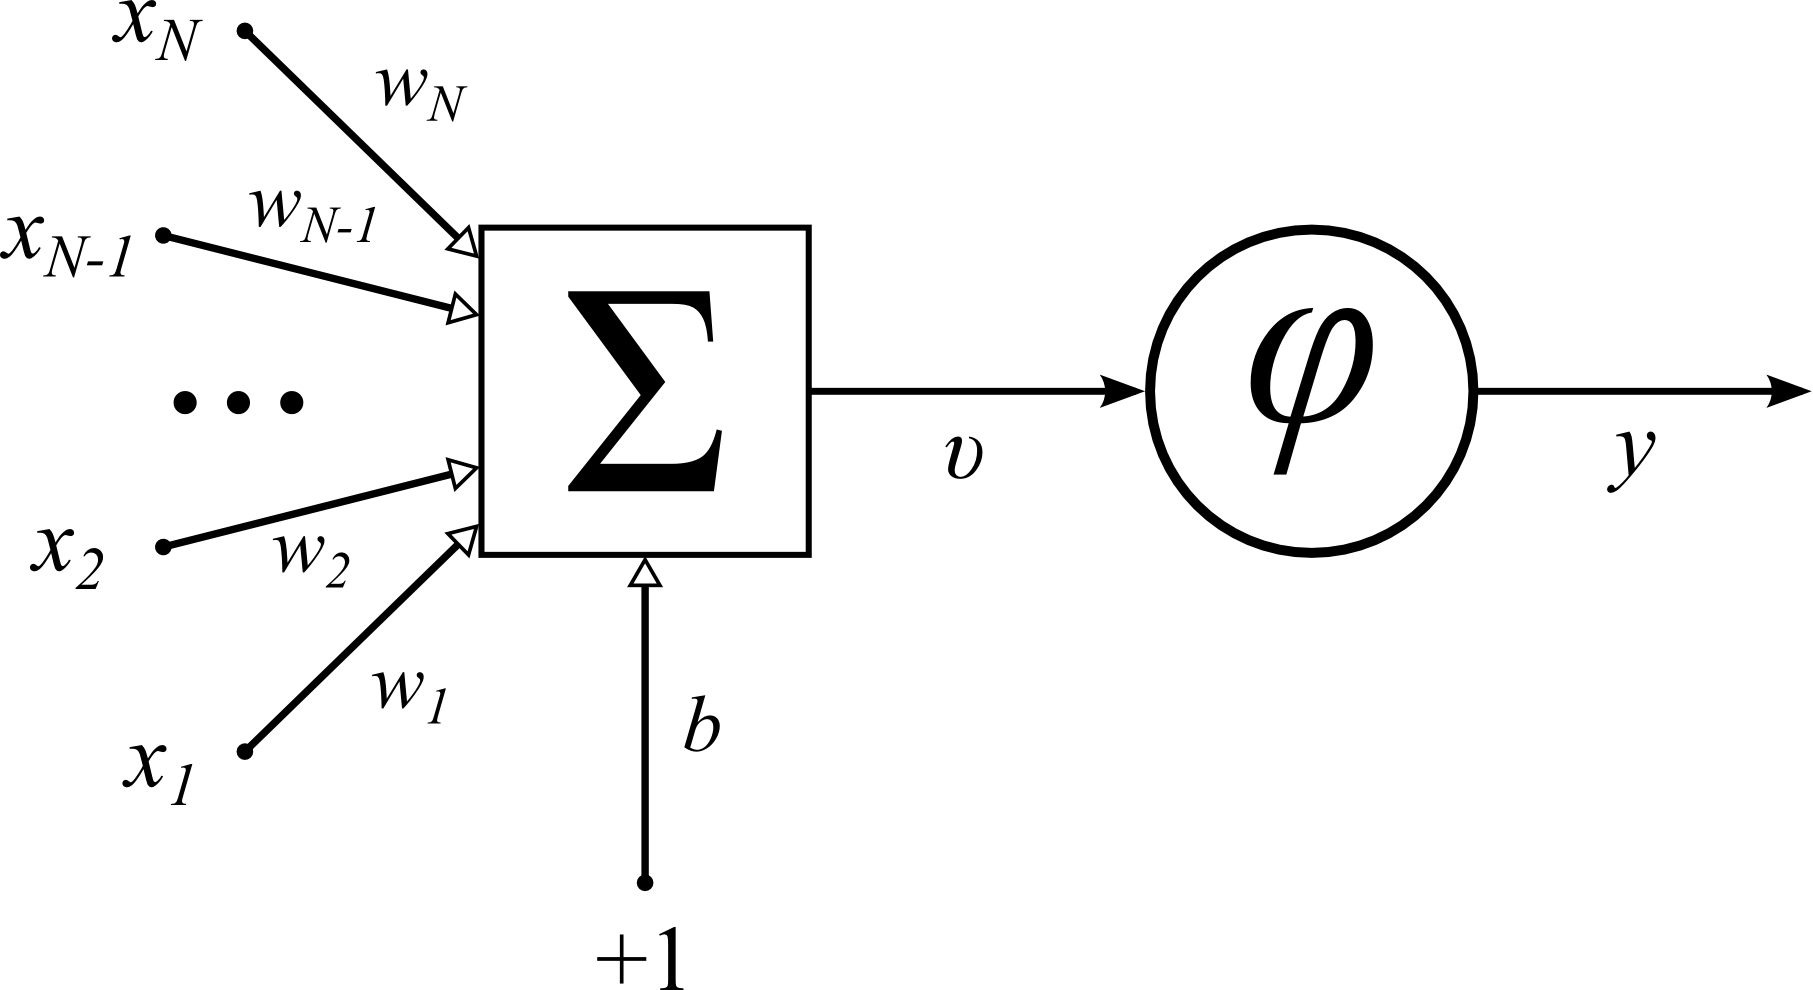
\includegraphics[width=11cm]{artificalNeuron.png}
	\caption{Схематическое представление искусственного нейрона}
	\label{fig:artificalNeuron}
\end{figure}

Математически эту модель можно записать в виде: $y = \phi( \sum_{i=1}^N w_i x_i + b)$.
В настоящее время чаще всего используется сигмоидальная функция активации, которая определяется как $\phi(\nu) = 1 / (1 + e^{-\alpha \nu})$, где $\alpha$ --- некоторый параметр, оптимальное значение которого находится эмпирически.

% мнослойный персептрон
Одной из самых простых моделей искусственных нейронных сетей является простая нейронная сеть с несколькими скрытыми слоями.
Такая нейронная сеть состоит из множества входных узлов, образующих входной слой, одного или нескольких скрытых слоев вычислительных нейронов и одного выходного слоя нейронов.
В такой сети каждый нейрон одного слоя соединён со всеми нейронами предыдущего и последующего слоёв.
Слой, состоящий из таких нейронов, называется полностью связанным слоем.
Входной сигнал распространяется по сети в прямом направлении, от слоя к слою без обратных связей, поэтому такая сеть является нейронной сетью прямого распространения или статической сетью.
Простые нейронные сети с несколькими скрытыми слоями могут применяться для решения широкого круга сложных задач.

Нейронные сети имеют возможность обучаться, в чем и заключается одно из главных их преимуществ перед традиционными методами \cite{nikolenko2017}.
Здесь обучение с учителем выполняется с помощью алгоритма обратного распространения ошибки, который является частным случаем алгоритма минимизации среднеквадратичной ошибки для случая отдельного линейного нейрона.
С математической точки зрения процесс обучения представляет собой нахождение оптимальных весовых коэффициентов, связывающих нейроны.
Лучше, если каждый уровень сети имеет определённый смысл.
Пример такого смыслового разделения представлен на рисунке \ref{fig:staticNeuronNetwork}.

\begin{figure}[h]
	\centering
	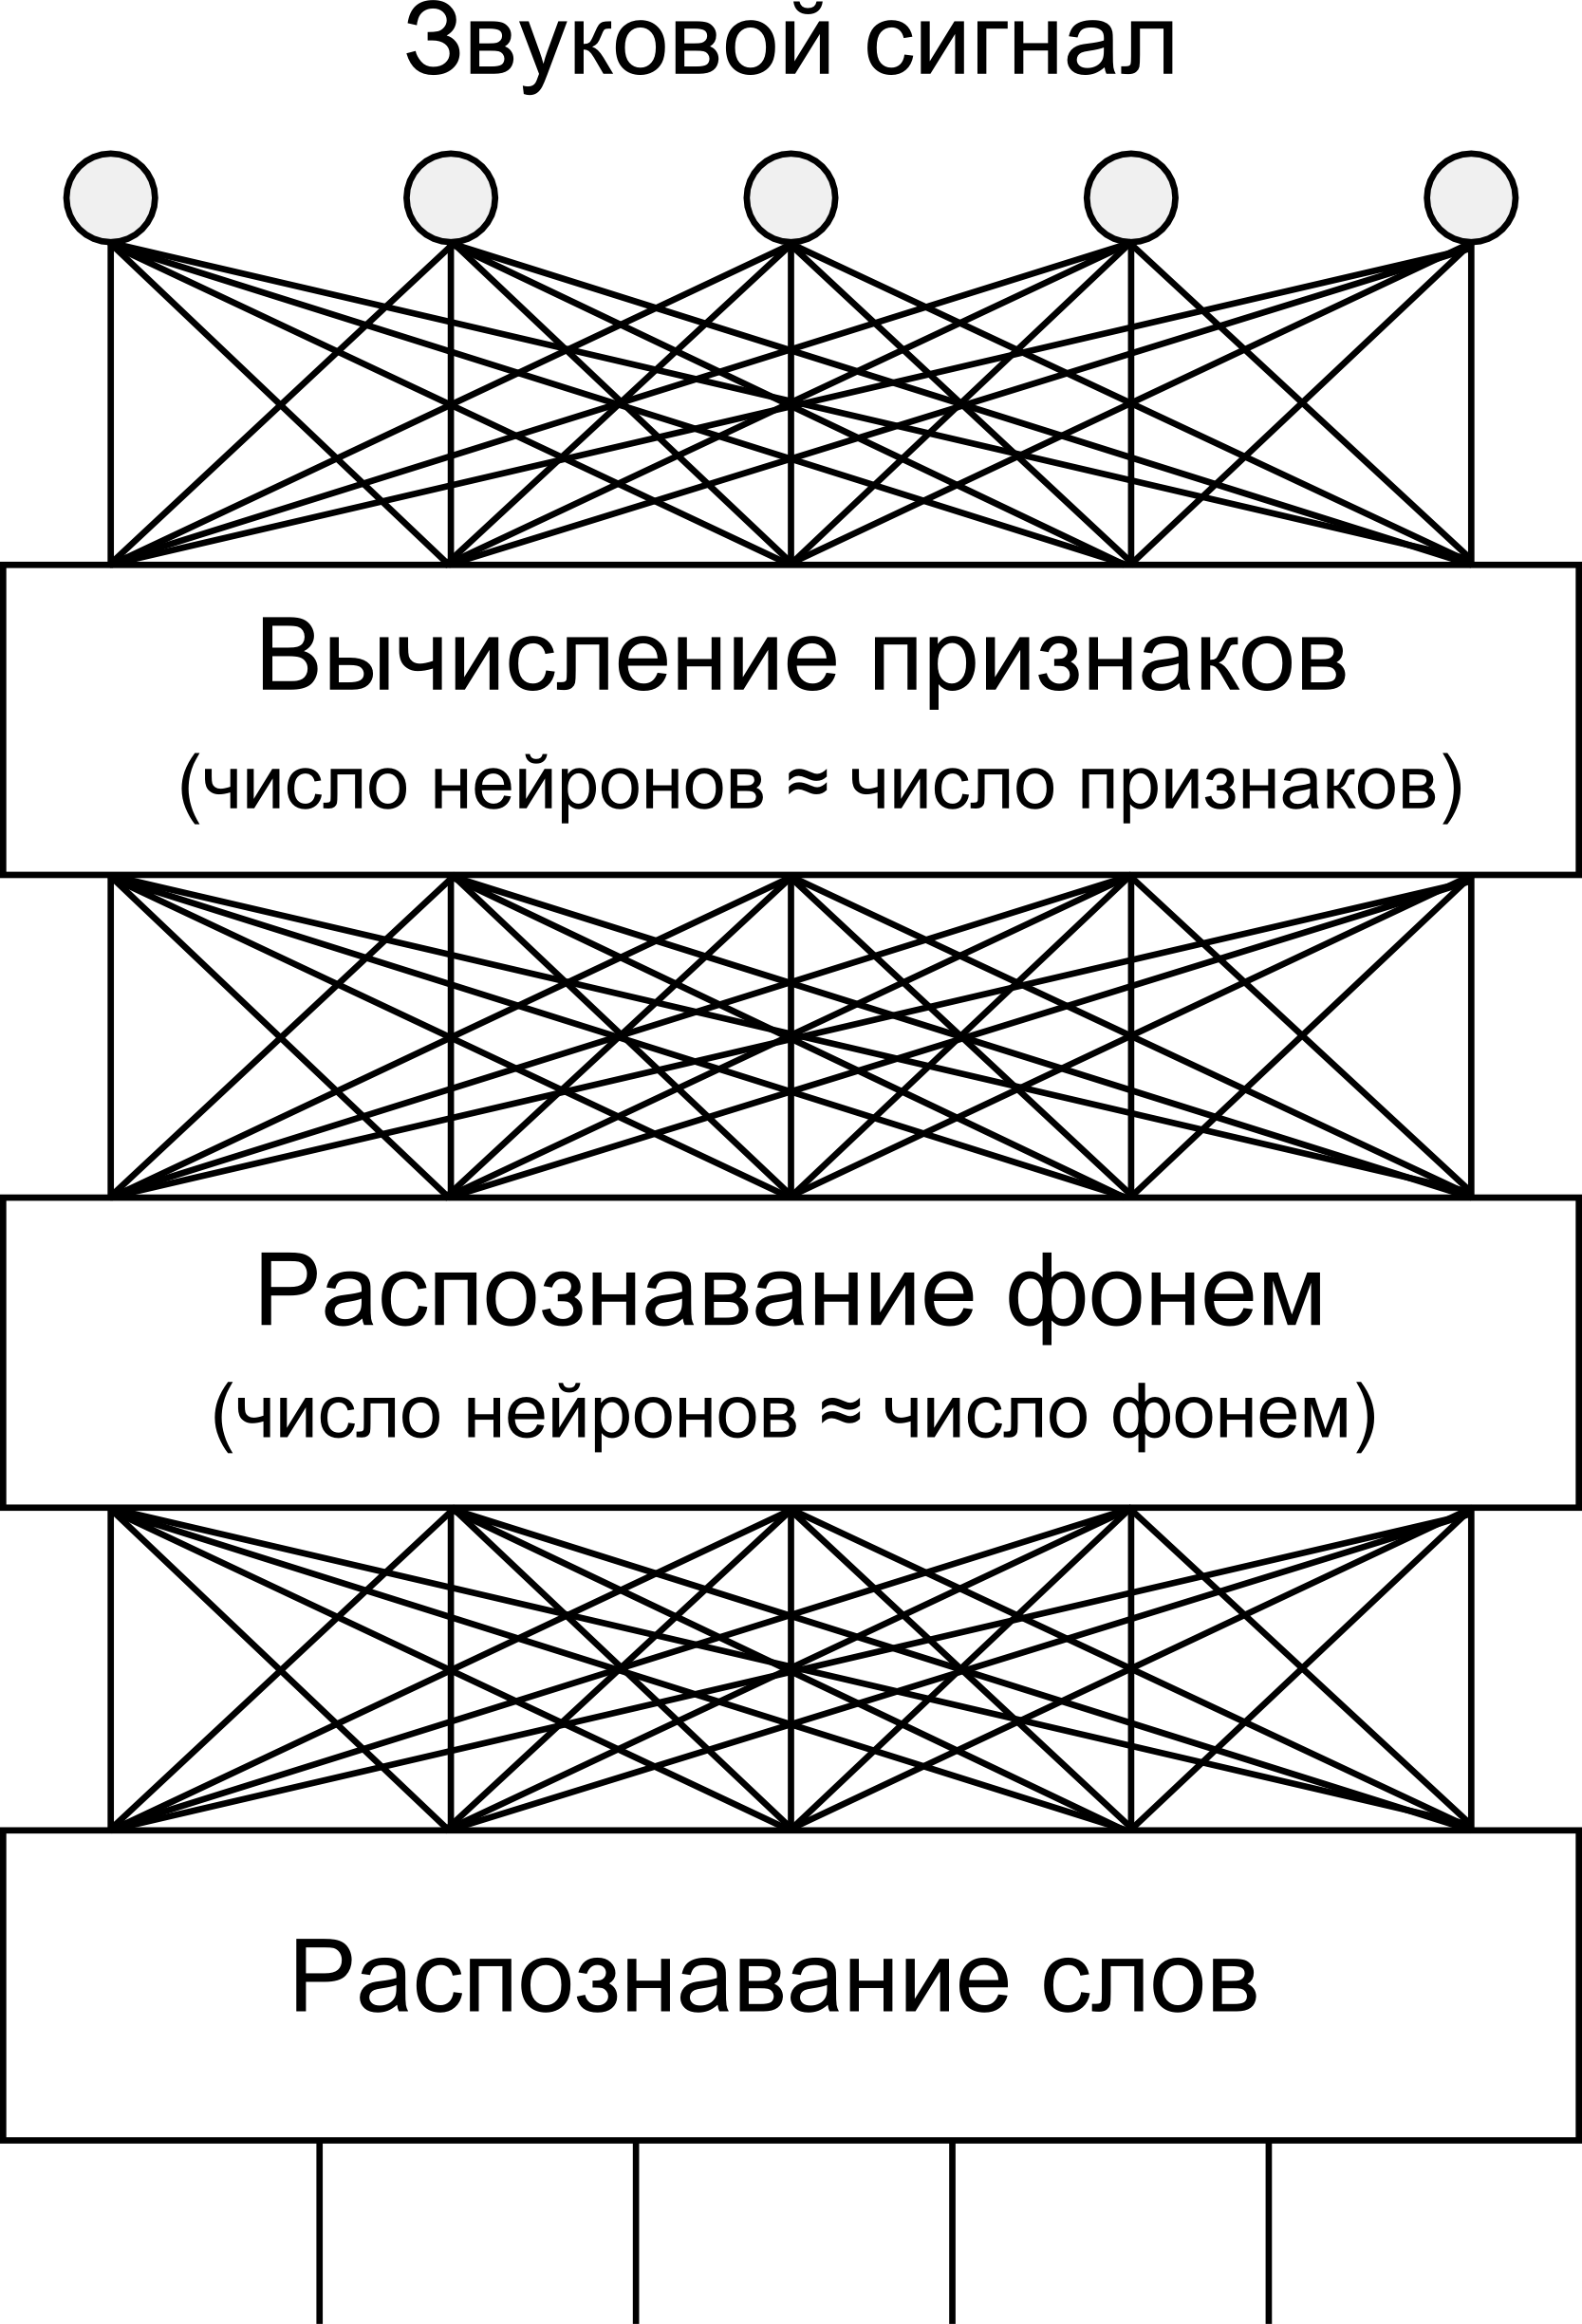
\includegraphics[width=9cm]{staticNeuronNetwork.png}
	\caption{Нейронная сеть прямого распространения с логически разделёнными уровнями}
	\label{fig:staticNeuronNetwork}
\end{figure}

% TDNN
В задачах распознавания речи также применяются искусственные нейронные сети с временными задержками или Time Delay Neural Network (TDNN).

По структуре они являются многослойной нейронной сетью прямого распространения.
Узлы данной сети также содержат временные задержки, что является главной особенностью данного типа искусственных нейронных сетей \cite{waibel1995phoneme}.
Пример внутреннего строения узла с $N$ задержками показан на рисунке \ref{fig:tdnnNode}.

\begin{figure}[h]
	\centering
	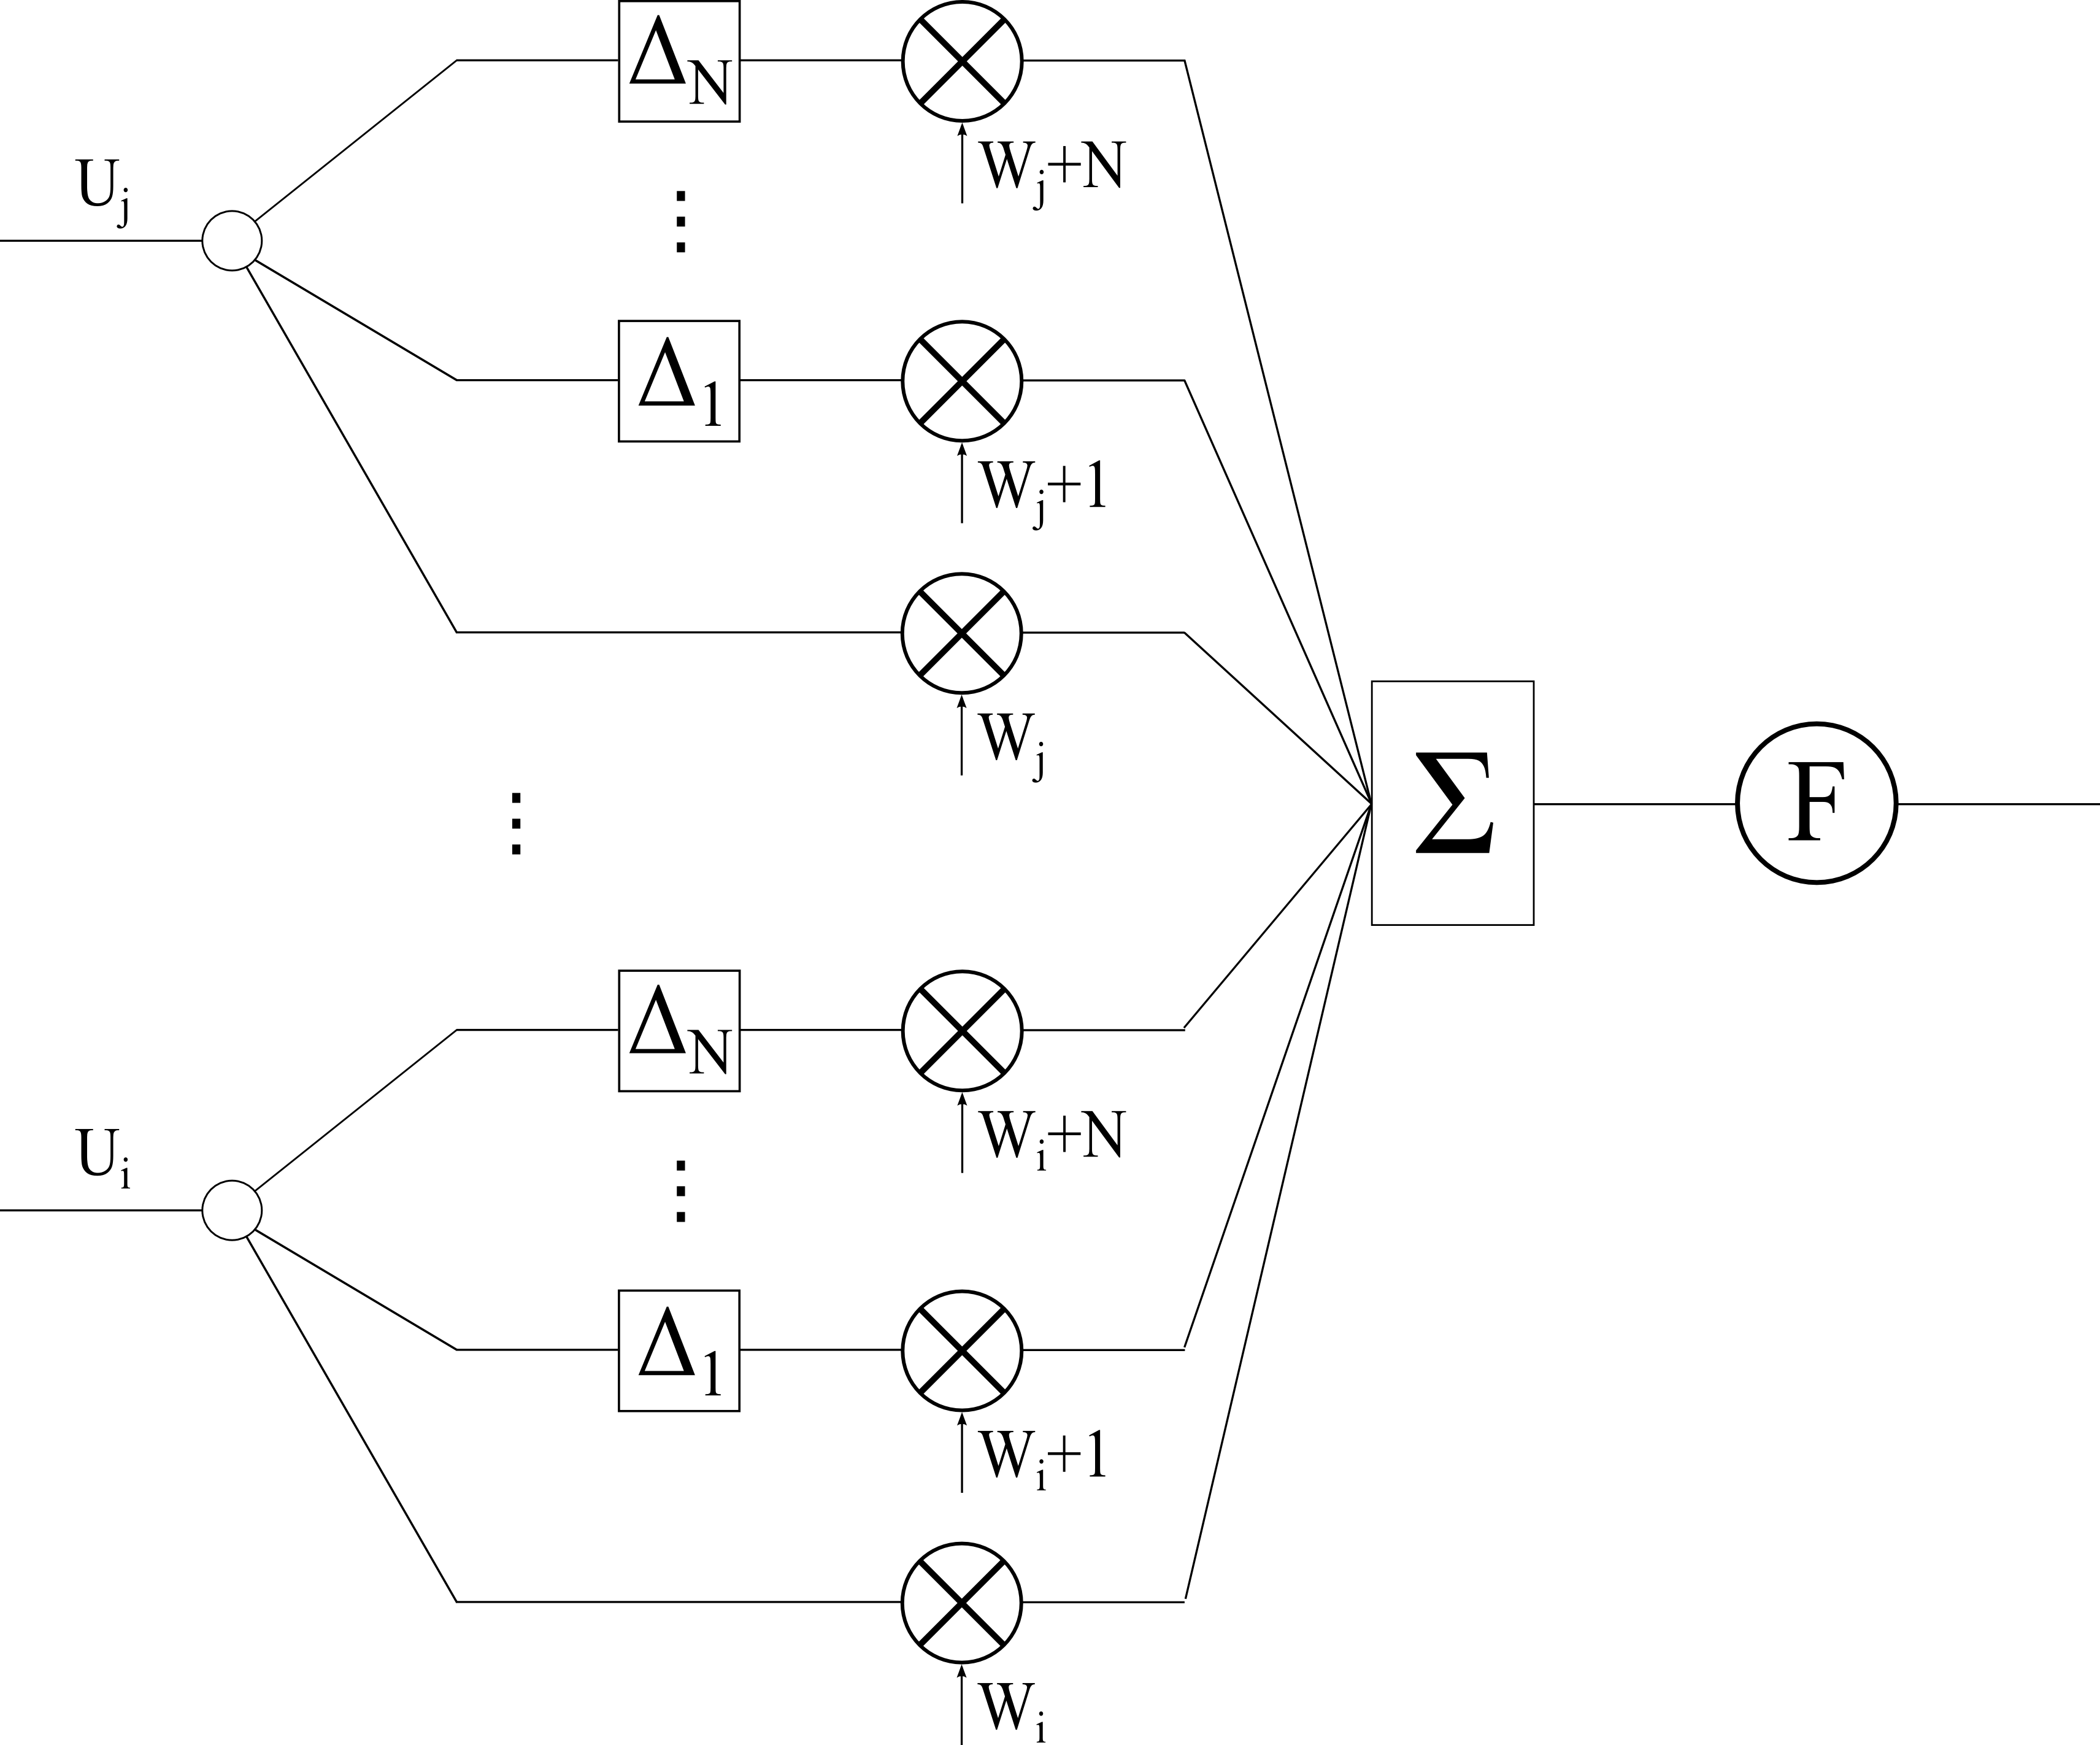
\includegraphics[width=12cm]{tdnnNode.png}
	\caption{Архитектура узла нейронной сети с временными задержками}
	\label{fig:tdnnNode}
\end{figure}

Входные узлы обозначены как $X_1, \dots, X_n$, далее к каждому входному значению применяется $k$ различных смещений $\Delta_1, \dots, \Delta_k$, величина которых выбирается из специфики решаемой задачи.
Таким образом, в TDNN встраивается кратковременная память.
После применения смещений полученные значения умножаются на соответствующие весовые коэффициенты $w_i^j$, в общем случае различные, где $i = \overline{1, n}$ и $j = \overline{1, k}$.
Далее в элементе $\Sigma$ производится суммирование всех слагаемых и затем применяется функция активации $F$.

В качестве примера использования нейронной сети с временными задержками можно рассмотреть задачу распознавания трёх фонем.
Структура сети для решения такой задаче приведена на рисунке \ref{fig:tdnnNetwork}.

\begin{figure}[h]
	\centering
	\includegraphics[width=10cm]{tdnnNetwork.png}
	\caption{Структура нейронной сети с временными задержками}
	\label{fig:tdnnNetwork}
\end{figure}

Из рисунка видно, что обработка входного параметрического портрета представляет собой прохождение входными узлами нейронной сети всего портрета от начала до конца с помощью скользящего по времени окна.
Узлы скрытых слоев сети эквивалентны скользящим детекторам признаков и способны находить искомые образы в любой области входных данных.
Выходные узлы имеют равные веса связей с каждым временным моментом последнего скрытого слоя, поэтому все моменты времени для таких детекторов являются равноправными.
Это позволяет нейронной сети быть инвариантной к временным сдвигам распознаваемых и эталонных образцов фонем, если эти временные сдвиги меньше размера входной последовательности сети.
Данные факты наряду с простой структурой сети дают возможность TDNN быть подходящим инструментом для распознавания речевых сигналов.

% LSTM
Ещё одним типом искусственных нейронных сетей, используемых для распознавания речи, является нейронная сеть с долгой краткосрочной памятью или Long Short-Term Memory (LSTM) \cite{hochreiter1997long}.
Данная архитектура является разновидностью рекуррентных нейронных сетей или Recurrent neural network (RNN).

У обычных нейронных сетей есть серьёзный недостаток --- они не умеют накапливать информацию о предыдущих события, а рекуррентные нейронные сети решают данную проблему.
В них присутствуют сохраняющие информацию циклы, другими словами блоки имеют связи сами с собой.
Из-за присутствия таких циклов рекуррентные сети выглядят довольно необычно и запутанно, но каждый цикл можно представить как несколько копий одного и того же блока.
Развёртка показана на рисунке \ref{fig:rnnBlock}, где видно, что развёрнутая сеть уже больше похожа на традиционные нейронные сети.

\begin{figure}[h]
	\centering
	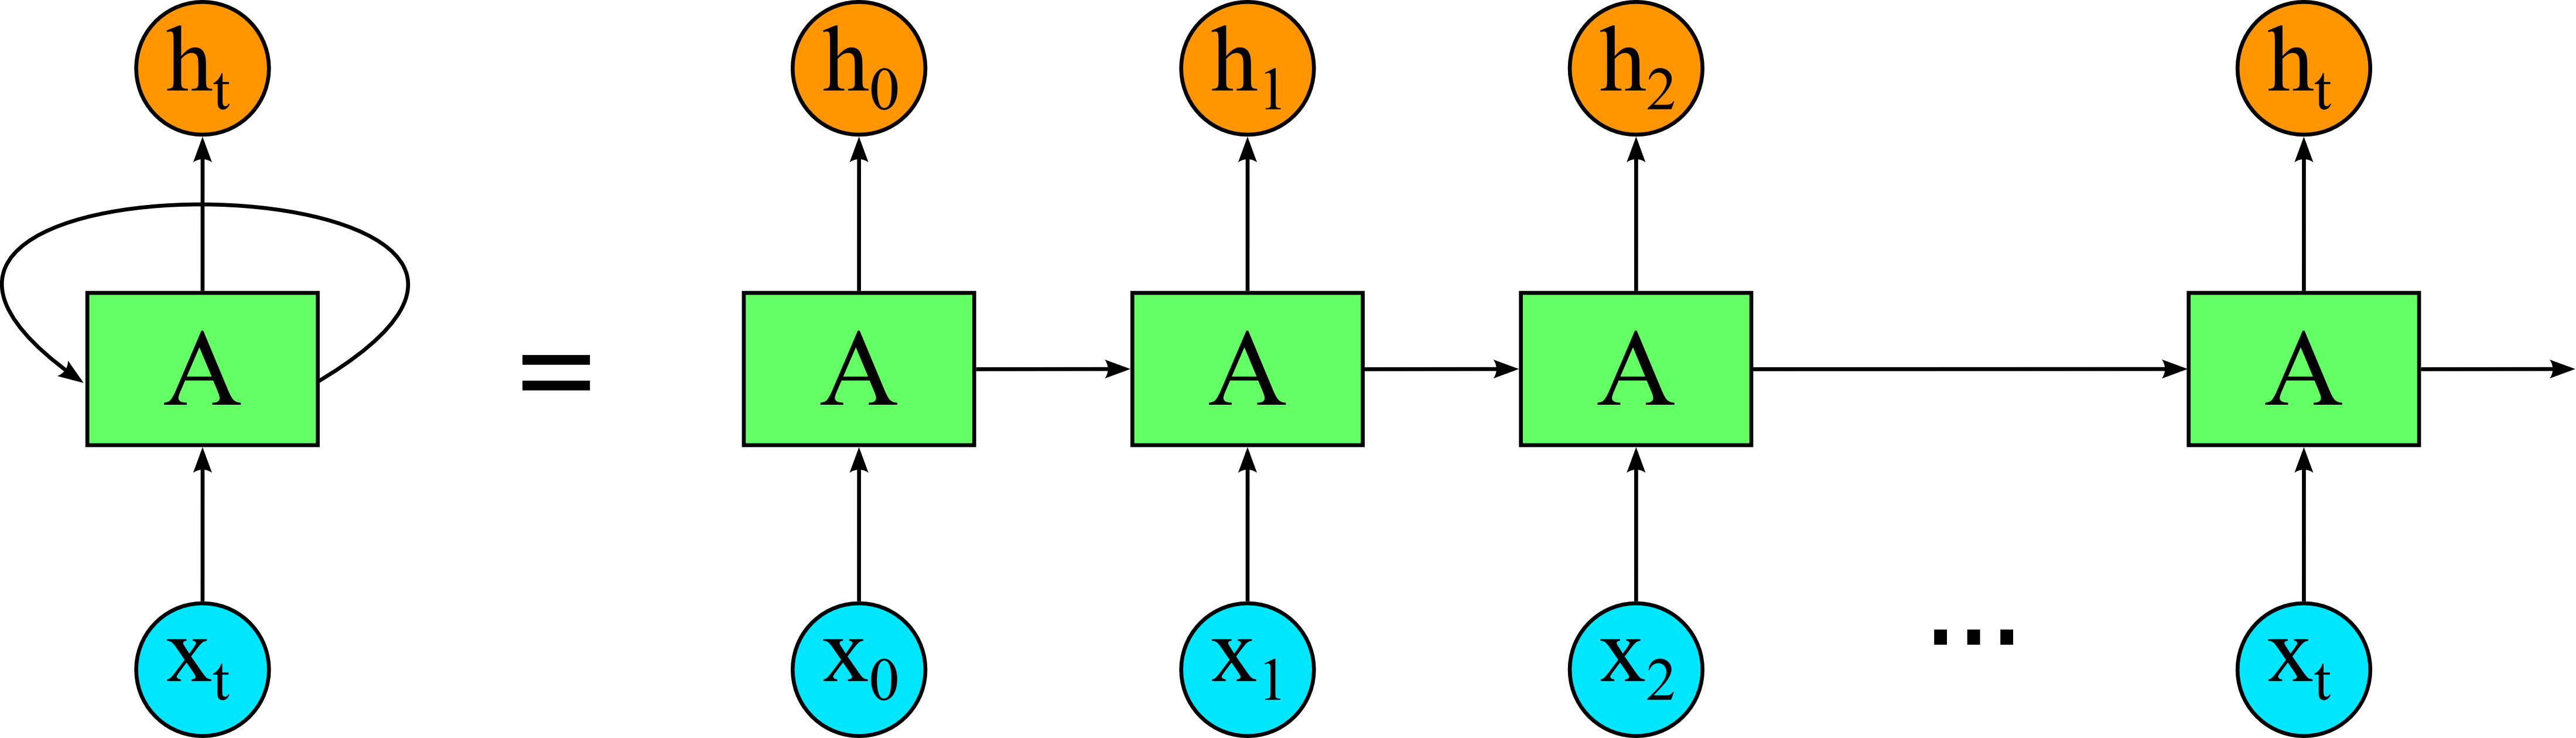
\includegraphics[width=16cm]{rnnBlock.png}
	\caption{Развёртка цикла рекуррентной нейронной сети}
	\label{fig:rnnBlock}
\end{figure}

Проблема RNN заключает в том, что она быстро <<забывает>> информацию, то есть с трудом строит долгосрочные зависимости между информацией в начале и в конце сигнала.
Нейронные сети c долгой краткосрочной памятью, как следует из их названия, были созданы как раз для решения данной проблемы.
Отличие LSTM от обычных RNN заключается в структуре блоков.
Блок стандартной рекуррентной сети как правило простой, например, один слой функции гиперболического тангенса.

LSTM-блоки обычно содержат 3 <<вентиля>>, которые используются для контроля потоков информации на входах и на выходах памяти блоков.
Блок с 3 вентилями: входным, выходным и вентилем забывания, приведён на рисунке \ref{fig:lstmBlock}.

\begin{figure}[h]
	\centering
	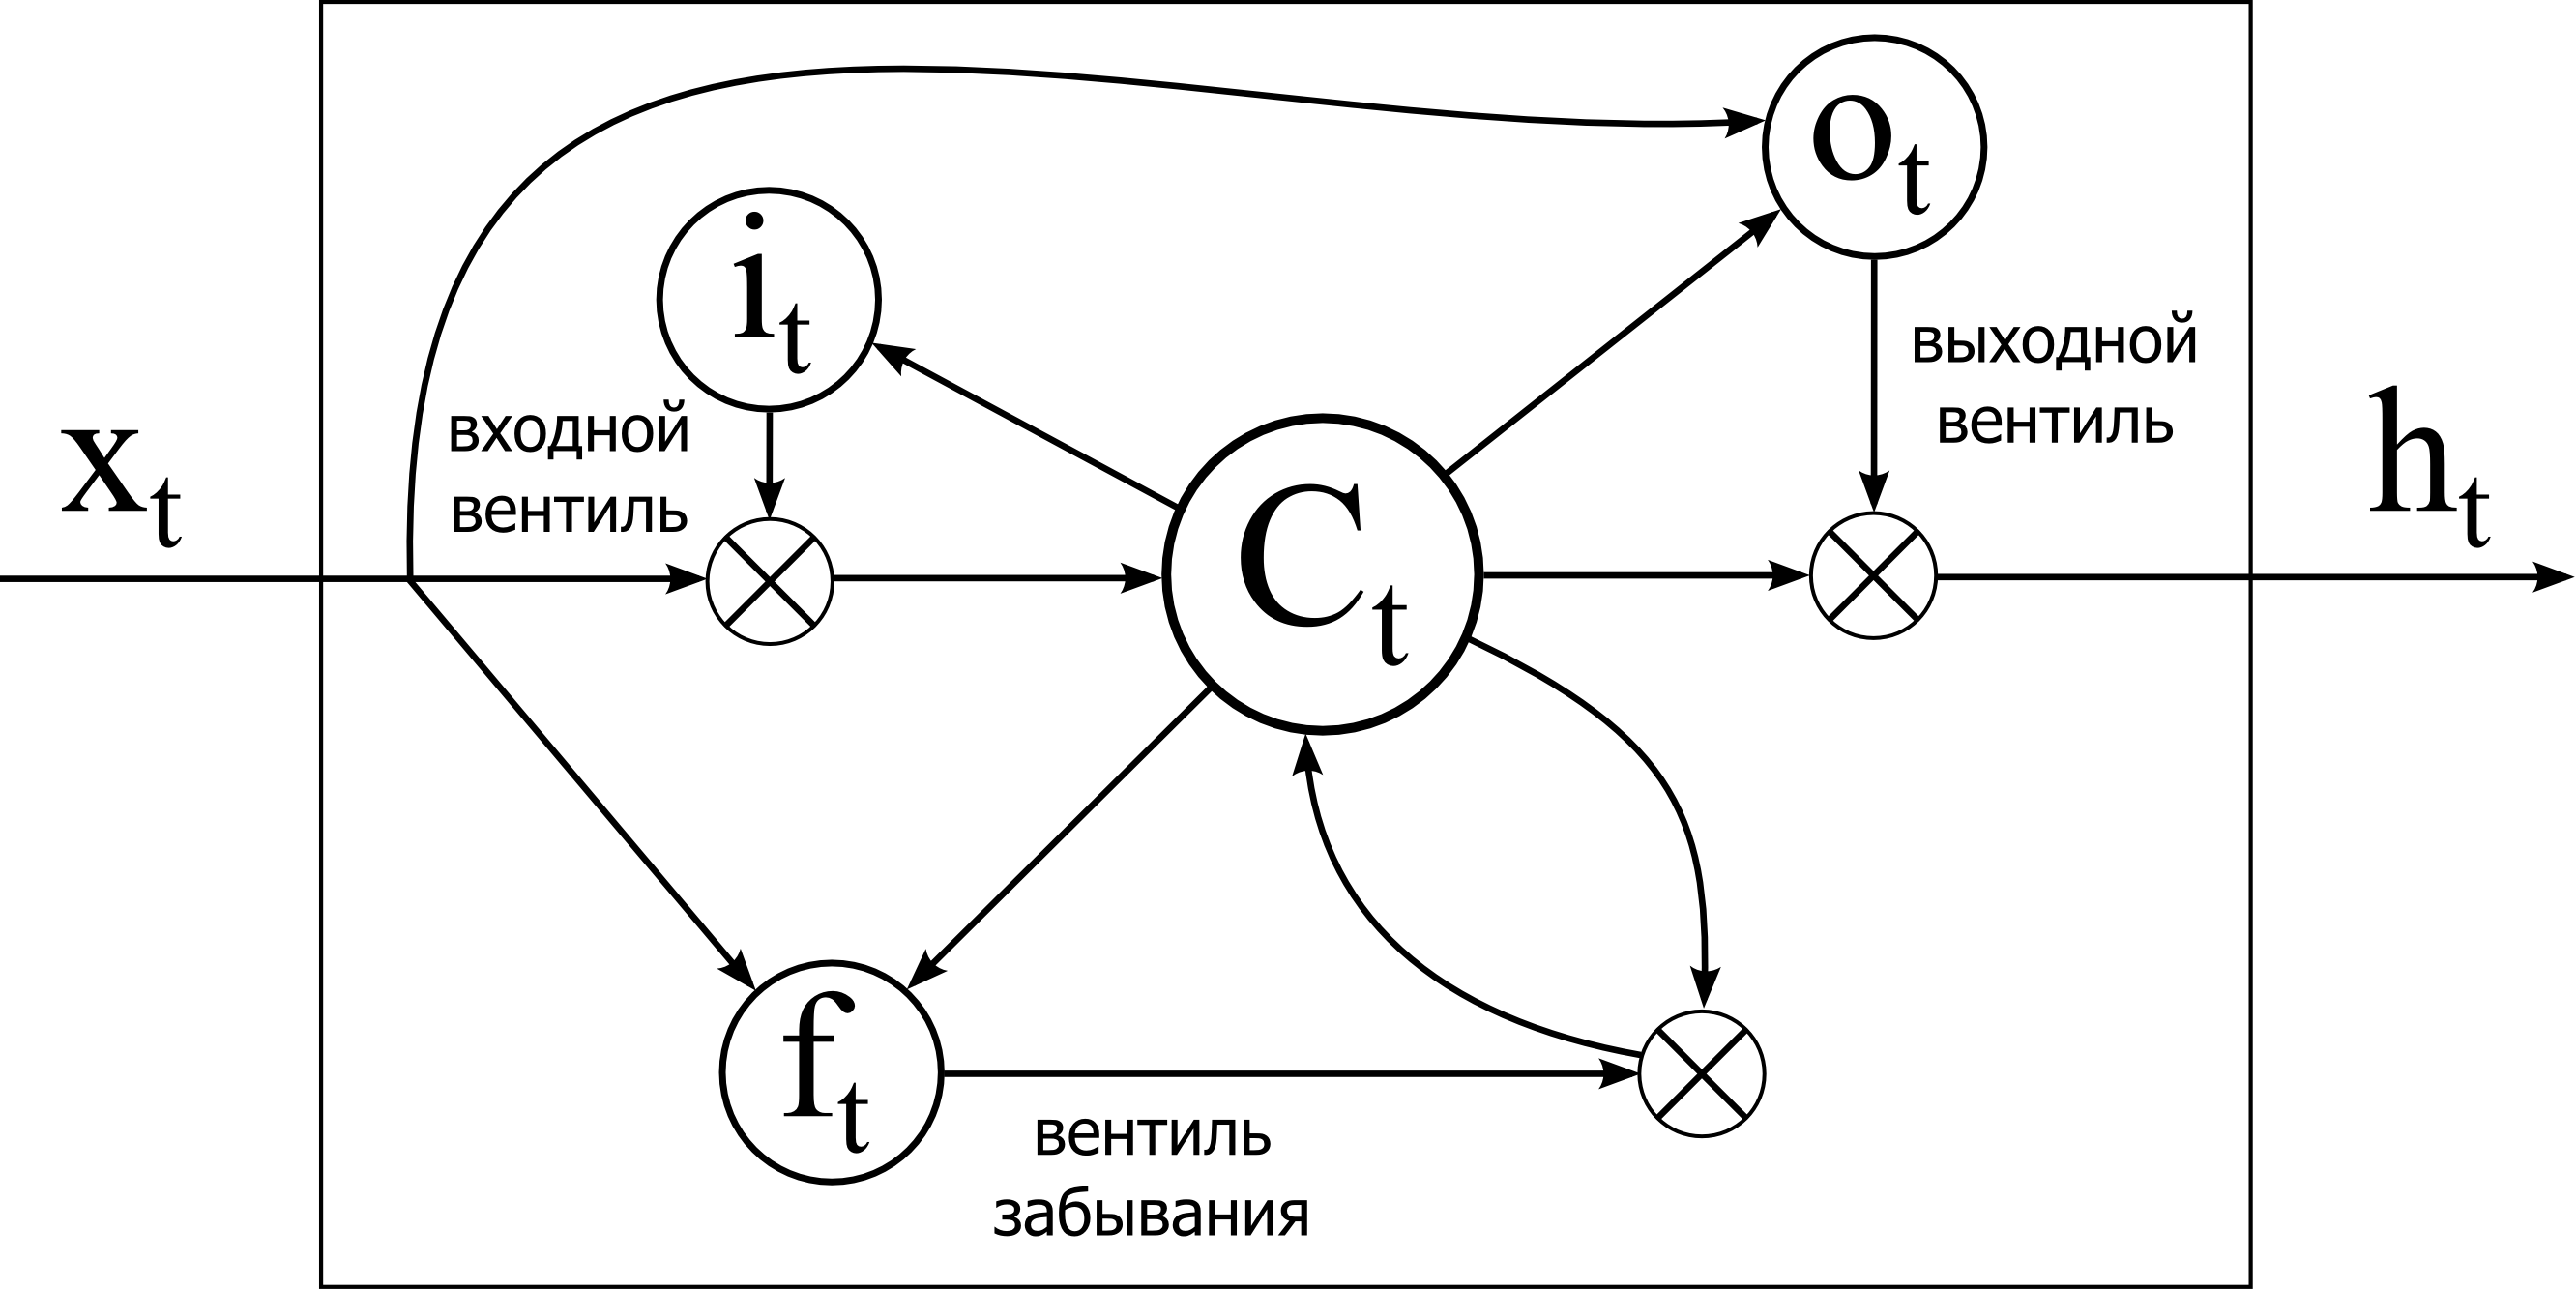
\includegraphics[width=14cm]{lstmBlock.png}
	\caption{Структура LSTM-блока с 3 вентилями}
	\label{fig:lstmBlock}
\end{figure}

Вентили реализованы в виде логистической функции для вычисления значения в диапазоне $[0, 1]$ и имеют в параметрах веса, которые подбираются в процессе обучения методом обратного распространения ошибки.
Умножение на это значение используется для частичного допуска или запрещения потока информации внутрь и наружу памяти.
Основная идея заключается в том, что старое значение следует забывать только тогда, когда появится новое значение достойное запоминания.

% сверточные нейронные сети
Другим классом искусственных нейронных сетей являются глубокие нейронные сети --- это нейронные сети прямого распространения с большим числом скрытых слоёв.
Одним из примеров глубоких нейронных сетей являются CNN (convolutional neural network, нейронные сети на основе свёртки), использующиеся при анализе изображений, распознавании речи и в других задачах \cite{lecun1995convolutional, abdel2014convolutional}.
В головном мозге человека были обнаружены клетки, имеющие различную функциональную нагрузку \cite{matsugu2003subject}.
Среди них были как простые клетки, которые реагировали на прямые линии, расположенные под различными углами, так и сложные клетки, которые активировались только при условии активации нескольких простых клеток.
Описанные выше искусственные нейронные сети как раз используют данное разделение функций между нейронами.
Общая схема работы CNN, описанная далее, показана на рисунке \ref{fig:cnn_typical}.

\begin{figure}[h]
	\centering
	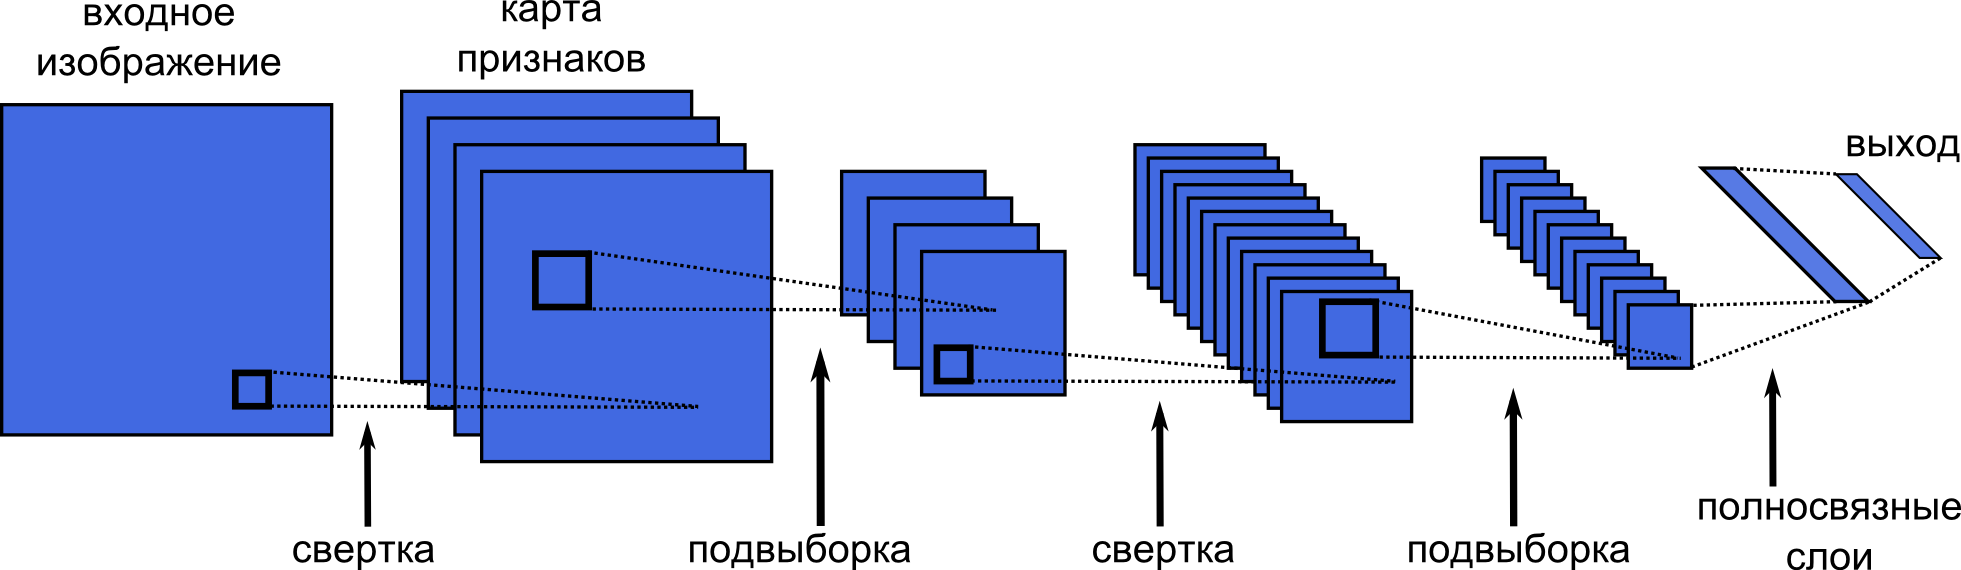
\includegraphics[width=1.0\textwidth]{cnn_typical.png}
	\caption{Общая схема работы CNN}
	\label{fig:cnn_typical}
\end{figure}

Так как изначально они были предложены для распознавания изображений, на вход подаётся один двухмерный массив (для черно-белых изображений) или несколько двухмерных массивов (для цветных изображений).
Такой формат входных данных отлично подходит для распознавания речи, так как в нём в качестве исходных данных также используется двухмерный параметрический портрет.
Входные массивы, также как и промежуточные массивы, называются картами признаков.

Далее вместо полностью связанных скрытых слоев используется другая структура сети, состоящая из чередующихся слоев свёртки и выборки.
На рисунке \ref{fig:convolution_pooling} приведено наглядное представление операции свёртки и операции выборки.

\begin{figure}[h]
	\centering
	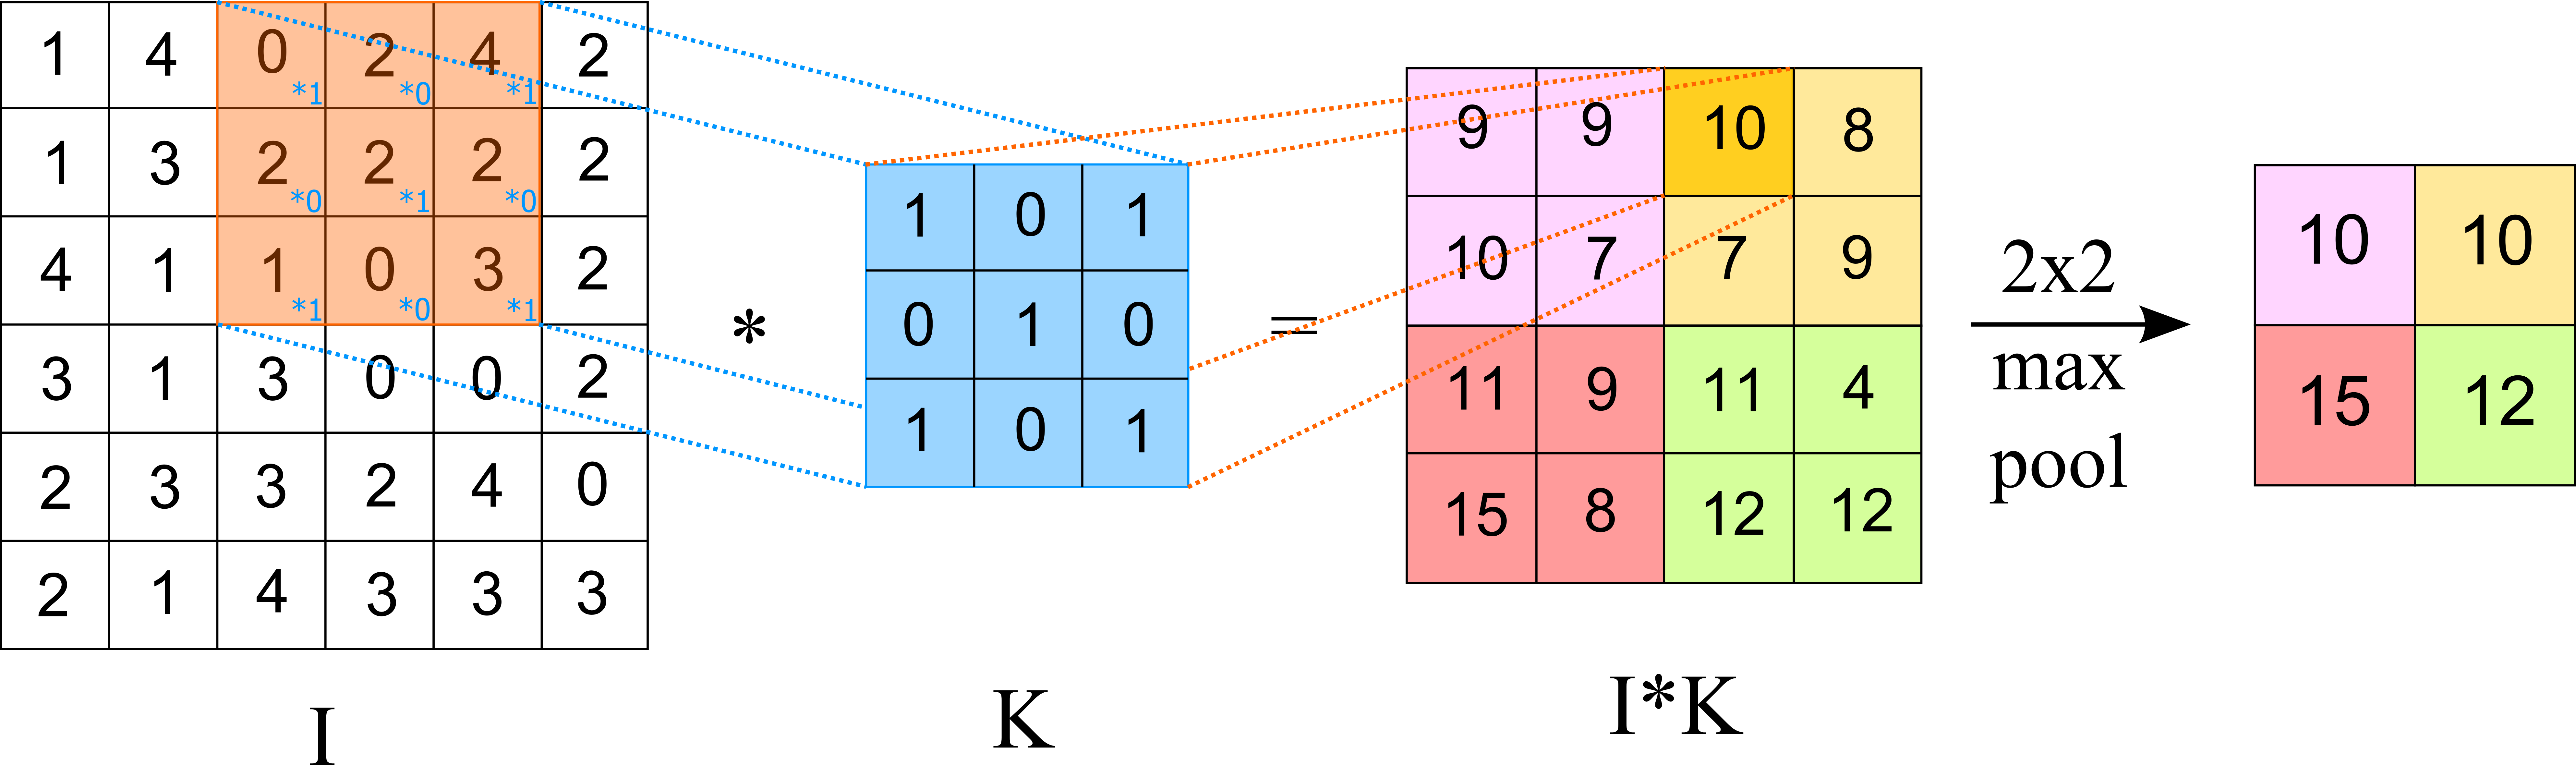
\includegraphics[width=1.0\textwidth]{convolution_pooling.png}
	\caption{Схема работы слоев свёртки и выборки в CNN}
	\label{fig:convolution_pooling}
\end{figure}

В операции свёртки каждый фрагмент карты признаков умножается на некоторую матрицу свёртки (ядро) поэлементно, а результат суммируется и записывается в соответствующую позицию выходной карты признаков.
В каждом слое может применяться набор из нескольких матриц сверки, при этом проход каждым из фильтров создаёт уникальную карту признаков.
Это делает искусственную нейронную сеть многоканальной, то есть имеется набор независимых карт признаков в каждом слое.
Операция выборки производит уменьшение размерности сформированных карт признаков, позволяя ускорить дальнейшие вычисления и обеспечить инвариантность к масштабу входного сигнала.

По мере прохождения слоев свёртки и выборки, карта признаков уменьшается в размере, но увеличивается количество каналов.
Далее, после прохождения всех слоев карта представляется в виде скаляра или вектора, но количество её каналов достигает нескольких десятков, сотен или даже тысяч.
На выходе нейронной сети дополнительно устанавливают один или несколько полностью связанных слоёв, на вход которым подаются все каналы из карты признаков.

Стандартным методом, используемым при обучении искусственных нейронных сетей, является алгоритм обратного распространения ошибки.
Также может быть использована любая функция активации нейронов.

%\newpage
%============================================================================================================================

\section{Обзор используемых в работе математических алгоритмов} \label{sect1_4}

В данном подразделе будут рассмотрены математические методы, используемые далее в предложенных алгоритмах.

%\newpage
%============================================================================================================================

\subsection{Методы математической статистики, необходимые для анализа свойств речевых сигналов} \label{sect1_4_1}

Существует несколько критериев согласия для проверки законов распределения случайной величины.
Это критерии согласия Колмогорова, Смирнова, $\chi^2$ Пирсона и другие.
В данной работе для проверки статистических гипотез будет использоваться критерий Пирсона, как один из наиболее часто употребляемых и широко описанных в литературе критериев для проверки закона распределения случайной величины \cite{panteleev2001}.

\textbf{Формирование критерия оценивания качества распознавания}

Сравнение распознаваемого слова с эталоном можно осуществить по критерию максимума коэффициента корреляции, оценка которого вычисляется по формуле 

\begin{equation}
\widehat{\rho}_{xe} = \frac{\sum_{n=1}^{N_s} (x_n - \widehat{m}_x)(e_n - \widehat{m}_e)}{\sqrt{\sum_{n=1}^{N_s} (x_n - \widehat{m}_x)^2 \sum_{n=1}^{N_s} (e_n - \widehat{m}_e)^2}},
\end{equation}
\begin{itemize}[align=left,leftmargin=1.8em,itemindent=0pt,labelsep=0pt,labelwidth=1.8em]
	\item[где] $x_n$, $e_n$, $n = 1, 2, \dots, N_s$ --- элементы матриц параметрического портрета рассматриваемого слова и эталона, преобразованные в одномерные массивы размерности $N_s = N_t N_f$;
	\item[] $\widehat{m}_x$, $\widehat{m}_e$ --- оценки средних параметрического портрета слова и эталона, вычисленные по множеству всех элементов, то есть 
	$\widehat{m}_x = \frac{1}{N_s} \sum_{n=1}^{N_s} x_n$, $\widehat{m}_e = \frac{1}{N_s} \sum_{n=1}^{N_s} e_n$.
\end{itemize}

При проверке гипотез и построении доверительных интервалов для коэффициентов корреляции часто используется Z-преобразование Фишера $z(\widehat{\rho}) = \frac{1}{2} \ln\left(\frac{1+\widehat{\rho}}{1-\widehat{\rho}}\right)$, где $\widehat{\rho}$ --- выборочный коэффициент корреляции.
Это преобразование даёт величину, распределение которой приближается к нормальному с математическим ожиданием $M[z] = \frac{1}{2} \ln\left(\frac{1+\rho}{1-\rho}\right)$ и дисперсией $D[z] = \frac{1}{n-3}$, где $n$ --- длина выборки, $\rho$ --- истинное значение коэффициента корреляции.

Далее в работе при сравнении двух параметрических портретов будет применяться именно Z-преобразование Фишера.

%============================================================================================================================

\subsection{Подстройка по длительности и динамическое программирование} \label{sect1_4_2}

При распознавании речевых команд путём сравнения их с эталонами требуется приведение временных масштабов двух сравниваемых слов в оптимальное соответствие.
Эффективное решение данной проблемы лежит в алгоритмах динамического программирования.
Алгоритмы такого типа являются динамическими алгоритмами трансформации временной шкалы.
Далее будет представлено описание работы данного алгоритма при распознавании отдельных слов.

Алгоритм динамической трансформации времени (ДТВ) основан на динамическом программировании.
Он вычисляет оптимальную последовательность трансформации времени между двумя временными рядами \cite{lama2010speech}.

Рассмотрим 2 последовательности векторов признаков различной длины: $A = \{a_1, a_2, \dots, a_i, \dots, a_n\}$ и $B = \{b_1, b_2, \dots, b_j, \dots, b_m\}$.
Допустим, что последовательность $A$ является эталоном, а последовательность $B$ --- входным словом.

Для начала рассчитаем величины локальных отклонений между элементами двух последовательностей.
Самым распространённым методом вычисления расстояния является расчёт абсолютного отклонения между значениями пары элементов.
В результате получится матрица расстояний, имеющая $m$ строк и $n$ столбцов общих членов: $dist_{ij} = |a_i - b_j|$, $i = \overline{1, n}$, $j = \overline{1, m}$.

Алгоритм динамического программирования определяется тем наблюдением, что в двумерной матрице наиболее оптимальный маршрут к точке $(i, j)$ должен быть проложен через точку $(i-1, j)$, или $(i-1, j-1)$, или $(i, j-1)$, как показано на рисунке \ref{fig:dynamicProgrammingPaths}.

\begin{figure}[h]
	\centering
	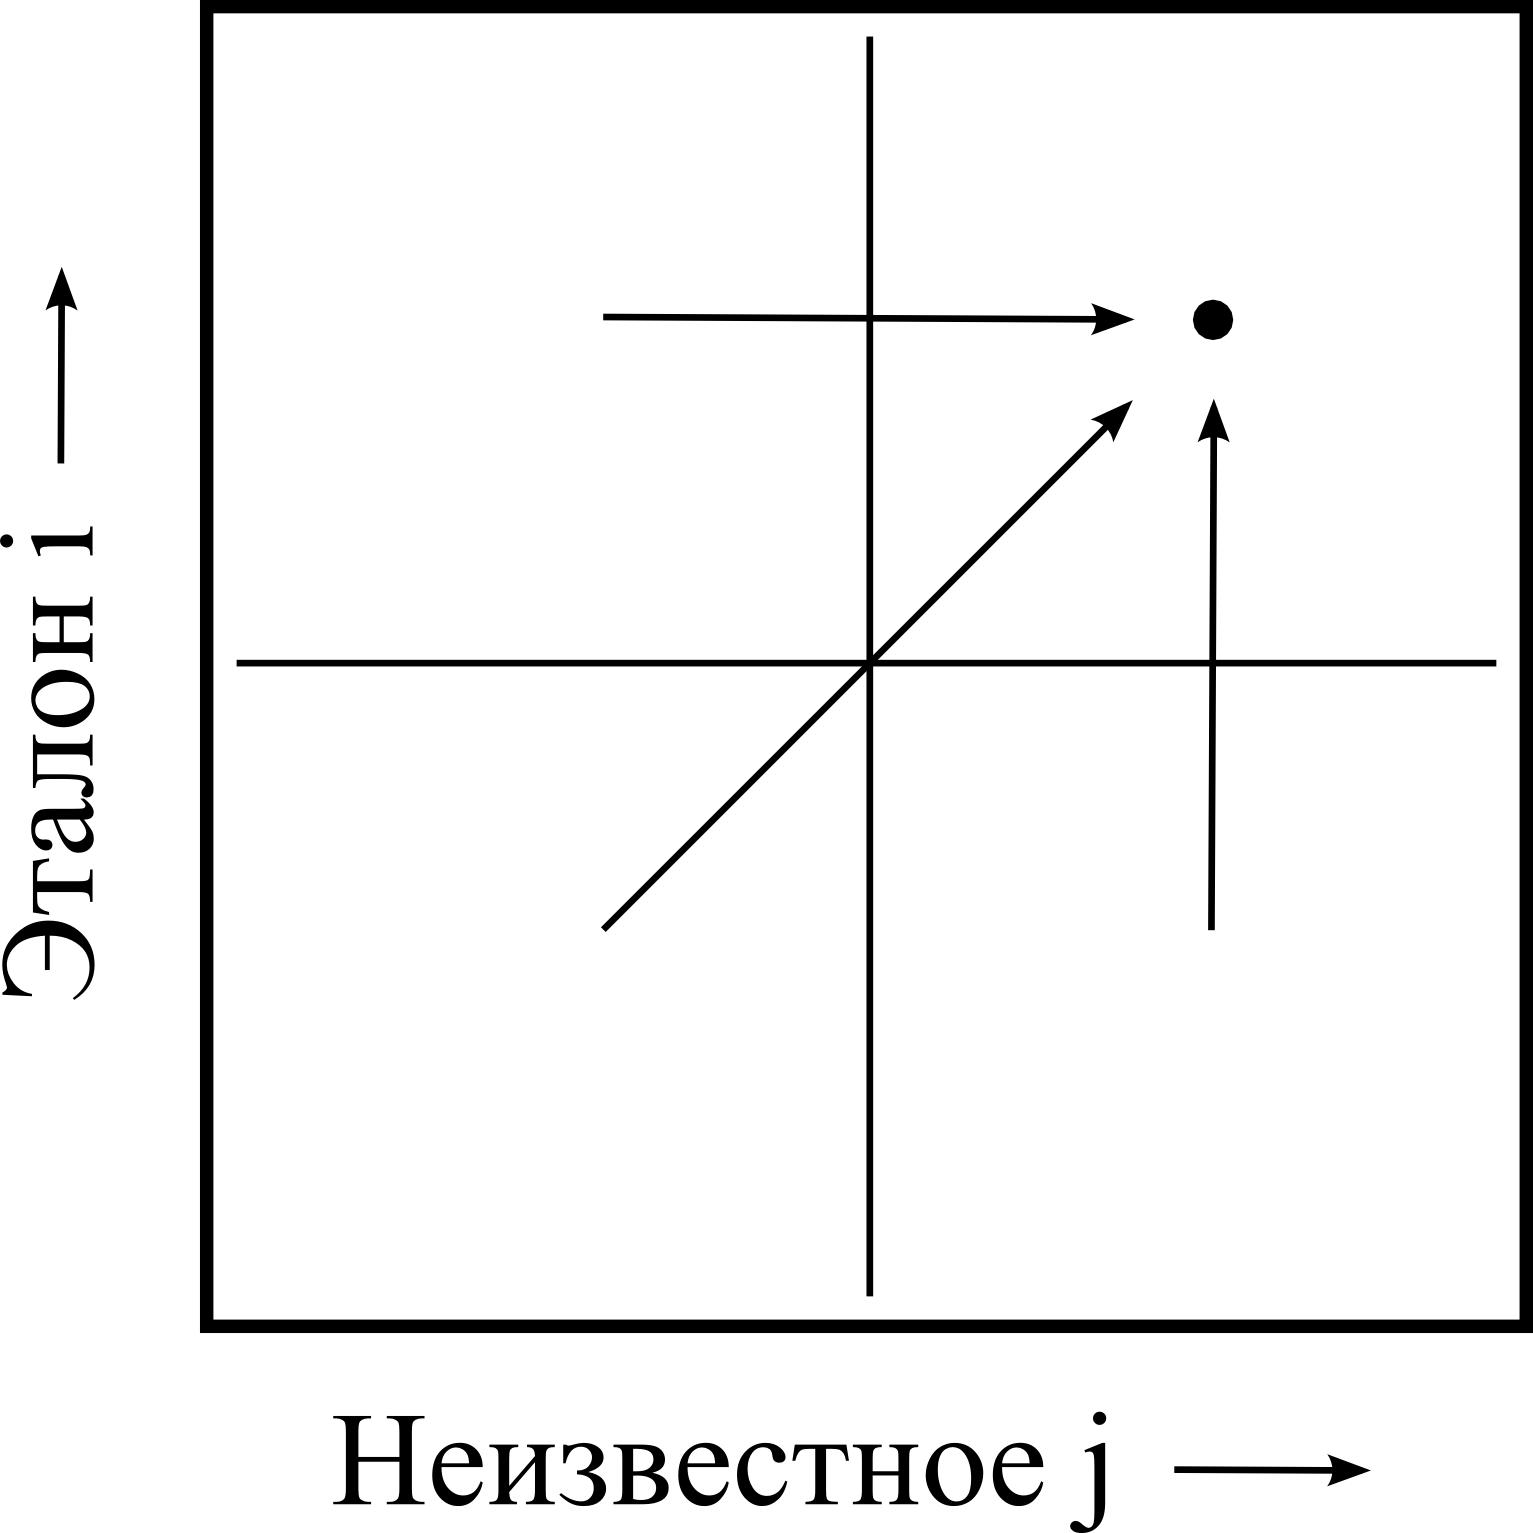
\includegraphics[width=6cm]{dynamicProgrammingPaths.png}
	\caption{Возможные варианты пути к $(i, j)$ в двумерной матрице}
	\label{fig:dynamicProgrammingPaths}
\end{figure}

Поэтому общий минимальный путь к точке $(i, j)$ определяется соотношением
\begin{equation}
D(i, j) = dist_{ij} + \min\{D(i-1, j); D(i-1, j-1); D(i, j-1)\},
\end{equation}
где $D(i, j)$ --- суммарное расстояние от точки $(1, 1)$ до точки $(i, j)$, а $dist_{ij}$ --- локальное расстояние (отклонение) в точке $(i, j)$, заданное выше.
\begin{itemize}[align=left,leftmargin=1.8em,itemindent=0pt,labelsep=0pt,labelwidth=1.8em]
	\item[где] $D(i, j)$ --- суммарное расстояние от точки $(1, 1)$ до точки $(i, j)$,
	\item[] $dist_{ij}$ --- локальное расстояние (отклонение) в точке $(i, j)$, заданное выше.
\end{itemize}

Длина пути от одной точки до следующей измеряется акустической аналогичностью эталона и неизвестного входного сигнала в этой точке.

Алгоритм рекурсивно вычисляет это расстояние элемент за элементом, чтобы определить минимальное суммарное расстояние $D(n, m)$ от начальной точки $(1, 1)$ до точки $(n, m)$ в верхнем правом углу.
Описанный путь позволяет получить временное выравнивание, в результате которого эталон становится максимально похож акустически на слово, которое было на входе.

На рисунке \ref{fig:dynamicProgrammingExample} схематически представлено выравнивание двух последовательностей на простом примере \cite{lea1980trends, gawali2010marathi}.

\begin{figure}[h]
	\centering
	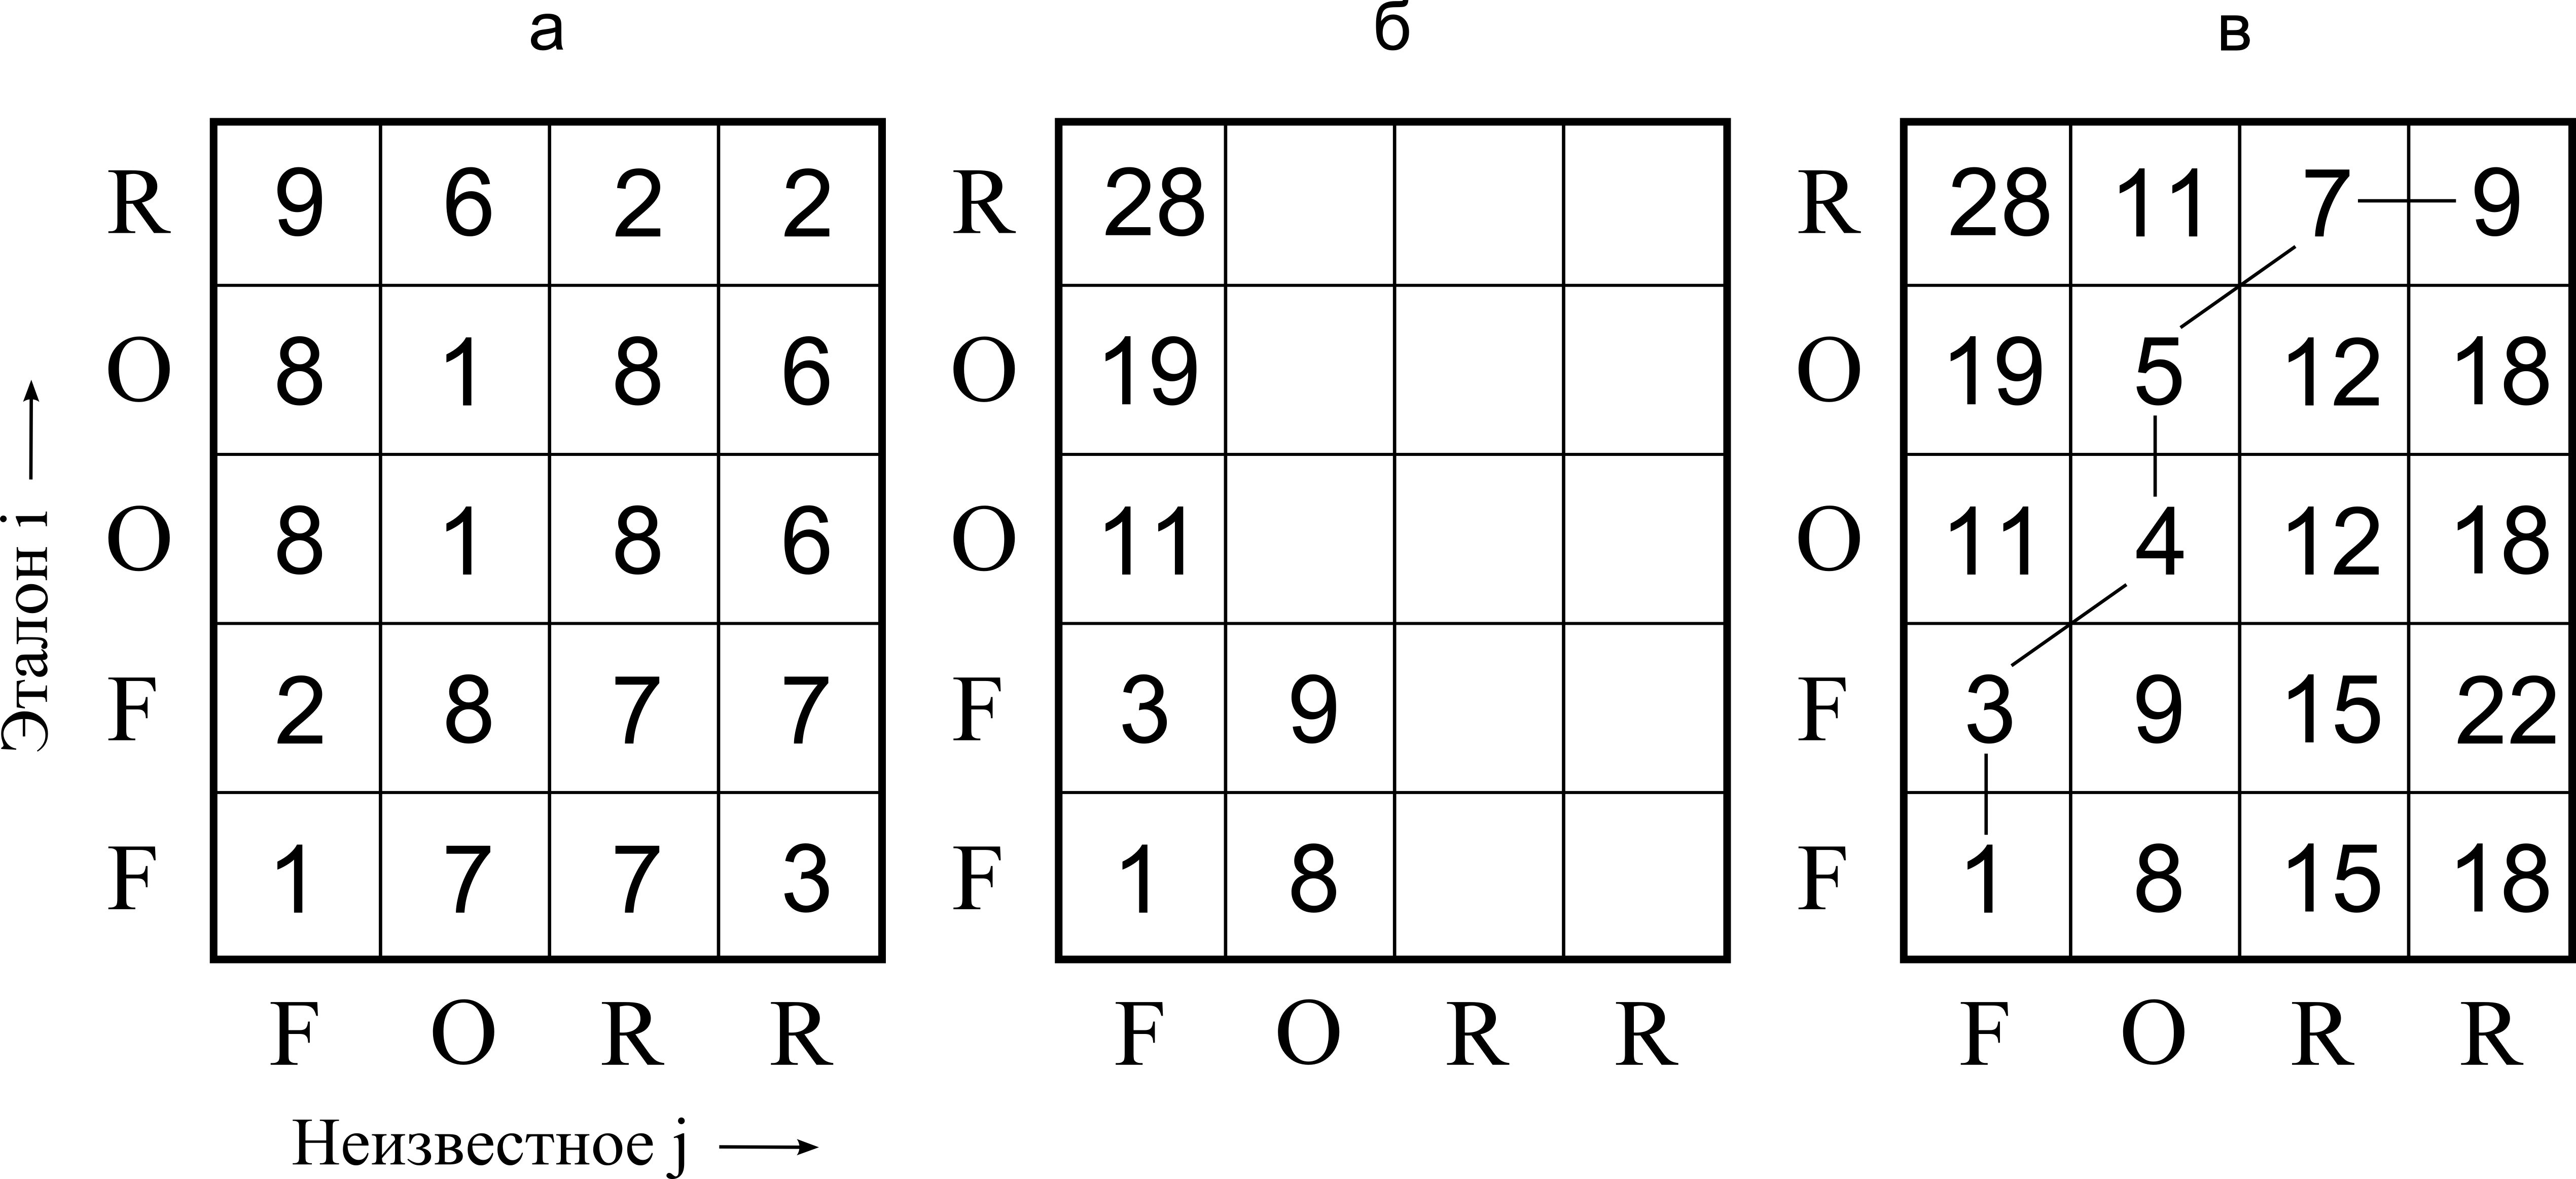
\includegraphics[width=16cm]{dynamicProgrammingExample.png}
	\caption{Пример динамического программирования: а) матрица подобия речевых звуков эталона и неизвестного сигнала; б) вычисление минимального общего расстояния до каждой точки по столбцам; в) окончательная матрица с общим совокупным расстоянием, равным 9}
	\label{fig:dynamicProgrammingExample}
\end{figure}

Длина последовательности эталона FFOOR равна $m = 5$, а длина распознаваемого слова FORR --- $n = 4$.
В первой части рисунка представлена матрица подобия элементов речевых сигналов эталона и распознаваемого слова.
В ней видно, что схожие элементы последовательностей имеют маленькие отклонения $dist_{ij}$, а различные элементы --- большие отклонения.
Все возможные пути, начало которых находится в нижнем левом углу и конец в верхнем правом углу дают совокупность возможных выравниваний неизвестного высказывания и соответствующего ему эталона.
Во второй части рисунка показан процесс построения суммарных расстояний $D(i, j)$.
А в третьей части рисунка показана полностью построенная матрица суммарных расстояний $D(i, j)$ и отмечен оптимальный путь до точки $(n, m)$.

В подразделе \ref{sect2_2} следующего раздела будет приведено подробное описание применяемых стандартного и модифицированного алгоритмов динамического программирования.

%\newpage
%============================================================================================================================

\subsection{Метод главных компонент} \label{sect1_4_3}

Для уменьшения размерности пространства используемых векторов без существенной потери информации используется метод главных компонент.
Метод главных компонент используется во многих областях от статистики до медицины \cite{aivazyan1989prikladnaya}.
Главные компоненты представляют собой ортогональную систему координат, в которой дисперсии компонент характеризуют их статистические свойства.

Пусть дан исходный набор векторов $\pmb{X}$ линейного пространства $\pmb{L}^p$.
Использование метода главных компонент даёт возможность перейти к базису пространства $\pmb{L}^{p'}$, $(p' \ll p)$, при котором первый вектор базиса сонаправлен с вектором, вдоль которого максимально значение дисперсии векторов изначального набора векторов.
Направление второго вектора базиса необходимо выбрать так, чтобы максимизировать значение дисперсии базовых векторов, проходящих вдоль него, при соблюдении условия ортогональности относительно первого вектора базиса.
Аналогично определяются остальные векторы базиса.

В итоге для того, чтобы максимально увеличить значение дисперсии изначального набора векторов вдоль первых компонент, называемых главными компонентами, были подобраны соответствующие направления векторов базиса.
Таким образом, основные показатели изменчивости базовых наборов векторов обусловлены характеристиками нескольких первых компонентов, вследствие чего возможно перейти к пространству с меньшей размерностью, исключив менее существенные компоненты \cite{aivazyan1989prikladnaya}.

Пусть имеется многомерное наблюдение $X_i = \begin{pmatrix} x_i^{(1)} \\ x_i^{(2)} \\ \vdots \\ x_i^{(p)} \end{pmatrix}$, $i = \overline{1, n}$.
В итоге, задачей является переход от количества признаков $p$ к $p'$.
Что можно реализовать в случае определения всех возможных нормированных линейных ортогональных комбинаций начальных показателей $z^{(j)}(X) = c_{j1} (x^{(1)} - \mu^{(1)}) + \dots + c_{jp} (x^{(p)} - \mu^{(p)})$, где $[\mu^{(1)}, \dots, \mu^{(p)}]'$ --- вектор средних для переменной $X$.
В качестве меры информативности $p'$-мерной системы показателей $(z^{(1)}(X), \dots, z^{(p')}(X))$ используется выражение $I_{p'}(Z(X)) = \frac{D(z_1) + \dots + D(z_{p'})}{D(x_1) + \dots + D(x_{p})}$, где $D(z)$ --- это операция вычисления дисперсии случайной величины.
Можно продемонстрировать, что соотношение, позволяющее рассчитать $p$ главных компоненты вектора $X$, возможно представить в виде $Z = LX$, где $Z = (z^{(1)}, \dots, z^{(p)})'$, $X = (x^{(1)}, \dots, x^{(p)})'$, а матрица $L$ состоит из строк $l_j = (l_{j1}, \dots, l_{jp})$, $j = \overline{1, p}$, являющихся собственными векторами ковариационной матрицы случайной величины $X$ $\Sigma = \sigma_{ij}$, $i,j = \overline{1, p}$, соответствующими собственным числам $\lambda_j$, $j = \overline{1, p}$.

Основные свойства главных компонент:
\begin{itemize}
	\item матрица $L$ является ортогональной, то есть $L L' = L' L = I$, где $I$ --- единичная матрица; 
	\item ковариационная матрица вектора главных компонент: $\Sigma_{Z} = L \Sigma L' = \begin{pmatrix} \lambda_1 & \dots & 0 \\ \vdots & \ddots & \vdots \\ 0 & \dots & \lambda_p \end{pmatrix}$;
	\item равенство сумм дисперсий исходных признаков и главных компонент;
	\item мера информативности метода $I_{p'}(Z(X)) = \frac{\lambda_1 + \lambda_2 + \dots + \lambda_{p'}}{\lambda_1 + \lambda_2 + \dots + \lambda_p}$, где $\lambda_1, \lambda_2, \dots, \lambda_p$ --- собственные числа ковариационной матрицы $\Sigma$ вектора $X$, расположенные в порядке убывания;
	следует использовать данный критерий для принятия решения о допустимости отбрасывания определённого числа наименее значимых главных компонент без существенного ущерба, с целью уменьшения показателя размерности исследуемого пространства.	
\end{itemize}

%\newpage
%============================================================================================================================

\subsection{Обзор методов численной оптимизации, метод покоординатного спуска} \label{sect1_4_4}

Задачи отыскания наибольших или наименьших величин часто возникают в науке.
Классическими методами решения задачи минимизации являются метод покоординатного спуска, градиентный метод и метод Ньютона. 

Метод покоординатного спуска применяется для решения экстремальных задач, в которых целевая функция либо не обладает нужной гладкостью, либо является гладкой, но вычисление производных слишком трудоёмко.
В таких случаях желательно иметь методы решения, которые используют лишь значения функции.
При этом является наиболее простым в реализации из всех методов локальной оптимизации.
Данный метод хорошо описан в литературе \cite{alekseeva2008}.

Хотя метод координатного спуска не требует знания градиента, сходимость можно гарантировать лишь для гладких функций.
Если целевая функция не является гладкой, то метод может не сходиться к множеству решений задачи. 

%\newpage
%============================================================================================================================

\subsection{Полиномиальная аппроксимация, полиномы Чебышёва} \label{sect1_4_5}

В математике существенную роль играет аппроксимация функций, то есть построение по заданной функции другой сходной, но более простой функции.
Часто возникающая задача --- это интерполяция, то есть восстановление функции по её табличным значениям.
Эффективное решение --- это приближение этой функции полиномами.
Интерполяция алгебраическими многочленами функции $f(x)$ на отрезке $[a, b]$ — это построение многочлена $P_n(x)$, степени меньшей или равной $n$, принимающего в узлах интерполяции $x_0, x_1, \dots, x_n$ значения $f(x_i)$: $P_{n}(x_{i})=f(x_{i}),\quad i=0, 1, \dots, n$.
Интерполяцией называют такую разновидность аппроксимации, при которой кривая построенной функции проходит точно через имеющиеся точки данных.

Задача о приближении функции ставится следующим образом: данную функцию $f(x)$ требуется заменить обобщённым полиномом $Q_m (x)$ заданного порядка $m$ так, чтобы отклонение функции $f(x)$ от обобщённого полинома $Q_m (x)$ на указанном множестве $X = \{x \}$ было наименьшим.
При этом полином $Q_m (x)$ в общем случае называется аппроксимирующим \cite{demidovich2013numerical}.

Распространённый на практике случай обычно заключается в том, что заданный порядок $m$ аппроксимирующего полинома $Q_m (x)$ значительно меньше числа узлов $n$.
Это объясняется тем, что степень многочлена, более высокая, чем необходимо для точного прохождения кривой через точки, другими словами $m > n$, нежелательна, так как приводит к бесконечному числу решений.
Значения $m \le n$, но при этом близкие к $n$, нежелательны из-за феномена Рунге --- эффекта нежелательных осцилляций, возникающего при интерполяции полиномами высоких степеней.
В этом случае необходимы некоторые методы осуществления приближения.
Метод наименьших квадратов является одним из вариантов меры отклонения.
Согласно этому методу за меру отклонения полинома $Q_m (x)$ от данной функции $f(x)$ на множестве точек $x_0, x_1, \dots, x_n$ принимают величину
\begin{equation}
S_m = \sum_{i=0}^{n} \left[ Q_m (x_i) - f(x_i) \right]^2,
\end{equation}
равную сумме квадратов отклонений полинома $Q_m (x)$ от функции $f(x)$ на заданной системе точек.

Одно из лучших приближений функции на заданном интервале может быть получено при использовании разложения с помощью полиномов Чебышёва \cite{de1963functions}.

Многочлены Чебышёва первого рода $T_n (x)$ задаются с помощью следующего рекуррентного соотношения:
\begin{equation}
\begin{gathered}
T_0 (x) = 1, \\
T_1 (x) = x, \\
\vdots \\
T_{n+1} (x) = 2x T_n (x) - T_{n-1} (x).
\end{gathered}
\end{equation}

Хотя также можно использовать и явную формулу для получения многочлена Чебышёва заданной степени:
\begin{equation}
T_n (x) = \sum_{k=0}^{\lfloor n/2 \rfloor} \binom{n}{2k} (x^2 - 1)^k x^{n-2k}.
\end{equation}

В математике последовательностью ортогональных многочленов называют бесконечную последовательность действительных многочленов $p_{0}(x),\ p_{1}(x),\ p_{2}(x),\ \ldots$, где каждый многочлен $p_{m}(x)$ имеет степень $m$, а также любые два различных многочлена этой последовательности ортогональны друг другу в смысле некоторого скалярного произведения, заданного в пространстве $L^{2}$.
Последовательность многочленов Чебышёва является ортогональной для скалярного произведения с весом $\frac{1}{\sqrt{1-x^2}}$.
Из ортогональности полиномов следует линейная независимость и единственность разложения функции по этим полиномам.
Многочлен Чебышёва $T_{m}(x)$ часто используется для аппроксимации функций как многочлен степени $m$, который меньше всего отклоняется от нуля на интервале $[-1, 1]$.

Полиномы Чебышёва могут быть использованы для аппроксимации экспериментальных данных функцией.
В первую очередь, это помогает снизить размерность исходных данных.
Кроме этого, они помогают отбросить лишние шумы, которые могут мешать при сравнении слова с эталоном.

Для приближения экспериментальных данных полиномами Чебышёва область определения данных должна быть линейно отображена в интервал ортогональности аппроксимирующих многочленов, в данном случае это многочлены Чебышёва, с интервалом ортогональности $[-1, 1]$:

\begin{equation}
l: X_i \rightarrow [-1, 1],
\end{equation}
\begin{itemize}[align=left,leftmargin=1.8em,itemindent=0pt,labelsep=0pt,labelwidth=1.8em]
	\item[где] $l$ --- линейное отображение,
	\item[] $X_i$ --- область определения точек.
\end{itemize}

Примером отображения $l$, ставящего в соответствие заданный интервал в область ортогональности многочленов, $l: [x_{\min}, x_{\max}] \rightarrow [-1, 1]$, может быть функция

\begin{equation}
l (x) = \frac{2x - (x_{\max} + x_{\min})}{x_{\max} - x_{\min}}.
\end{equation}

%\newpage
%============================================================================================================================

\subsection{Метод комитетов} \label{sect1_4_6}

Метод комитетов представляет собой подход к решению различных задач распознавания, который объединяет принципы линейного разделения классов и вычисления коллективных решений \cite{senko}.
Для простоты рассмотрим задачу распознавания с двумя возможными классами $C_1$ и $C_2$.
Пусть $\Phi = \{f_1(\bar{x}), \dots, f_r(\bar{x})\}$ является набором линейных функций вида

\begin{equation}
f_i(\bar{x}) = a_1^i x_1 + \dots + a_n^i x_n,
\end{equation}
где $\bar{x} = (x_1, \dots, x_n)$ --- это вектор используемых для распознавания признаков, $(a_1^i, \dots, a_n^i)$ является вектором вещественных параметров, задающих линейную функцию $f_i(\bar{x})$.
\begin{itemize}[align=left,leftmargin=1.8em,itemindent=0pt,labelsep=0pt,labelwidth=1.8em]
	\item[где] $\bar{x} = (x_1, \dots, x_n)$ --- это вектор используемых для распознавания признаков,
	\item[] $(a_1^i, \dots, a_n^i)$ является вектором вещественных параметров, задающих линейную функцию $f_i(\bar{x})$.
\end{itemize}

Каждая из функций набора $\Phi$ рассматривается в качестве отдельного линейного классификатора, который относит объект с описанием $\bar{x}$ в класс $C_1$, если $sgn [f_i(\bar{x})] > 0$, и в класс $C_2$ в противном случае.

Допустим, что для классификации произвольного заданного объекта $\omega$, который имеет описание $\bar{x}$, применяется следующее решающее правило метода комитетов:

\begin{itemize}
	\item объект $\omega$ с описанием $\bar{x}$ относится в класс $C_1$, если выражение $\sum_{i=1}^{r} sgn [f_i(\bar{x})] > 0$;
	\item объект $\omega$ с описанием $\bar{x}$ относится в класс $C_2$, если выражение $\sum_{i=1}^{r} sgn [f_i(\bar{x})] < 0$;
	\item в случае, если величина $\sum_{i=1}^{r} sgn [f_i(\bar{x})] = 0$, то происходит отказ от распознавания.
\end{itemize}

Набор функций $\Phi$ называется комитетом, если решающее правило метода комитетов позволяет правильно классифицировать объекты обучающей выборки.

Метод, основанный на поиске оптимальных комитетов, реализует кусочно-линейную разделяющую поверхность, что потенциально позволяет производить распознавание линейно неразделимых классов.
Процесс обучения сводится к поиску оптимальных параметров $a_i^j$, $i = \overline{1, r}$, $j = \overline{1, n}$ в функциях из комитета.
Теоретически показано существование комитета для непротиворечивых данных \cite{mazurov1990method}.

%\newpage
%============================================================================================================================

\clearpage
